\documentclass[conference]{IEEEtran}
\IEEEoverridecommandlockouts
% The preceding line is only needed to identify funding in the first footnote. If that is unneeded, please comment it out.
\usepackage{cite}
\usepackage{amsmath,amssymb,amsfonts}
\usepackage{algorithmic}
\usepackage{graphicx}
\usepackage{textcomp}
\usepackage{xcolor}
\def\BibTeX{{\rm B\kern-.05em{\sc i\kern-.025em b}\kern-.08em
    T\kern-.1667em\lower.7ex\hbox{E}\kern-.125emX}}


\newcommand{\vectorsym}[1]{\ensuremath{\mathbf{#1}}}
\newcommand{\xextremum}{\ensuremath{x_{\mathrm{ext}}}}
\newcommand{\ccrit}{\ensuremath{c_{\mathrm{crit}}}}
\newcommand{\agentimpact}{\ensuremath{e}}
\newcommand{\empowerment}{\ensuremath{\mathfrak{E}}}
\newcommand{\sustainableempowerment}{\ensuremath{\empowerment^{\mathrm{sust}}}}
\newcommand{\setsymbol}[1]{\ensuremath{\mathcal{#1}}}
\newcommand{\stateset}{\ensuremath{\setsymbol{S}}}




% Daniel's comments
%\newcommand{\dpnote}[1]{{\color{magenta} \fbox{#1 \ref{undefined-ref-remove-when-fixed}}}}
\usepackage{ifthen}
\newsavebox{\laterrefbox}
\newlength{\tempwidth}
\newcommand{\dpnote}[1]{
  \sbox{\laterrefbox}{#1}%
  \ifthenelse{\lengthtest{\wd\laterrefbox > \linewidth}}
  {\setlength{\tempwidth}{\linewidth}
   { \color{magenta}
    \fbox{
        \begin{minipage}{0.9\linewidth}
          \textsl{\small #1}
        \end{minipage}
      }
    }
  }
  {{\color{magenta}\fbox{\textsl{\small #1}}}}
%   \fbox{\fbox{
%   \begin{minipage}{7cm}
%     \textsl{\small #1}
%   \end{minipage}%
%   }}%
  {\color{magenta} \ref{undefined-ref-remove-when-fixed}}%
}

\begin{document}

\title{Quantifying Sustainability in a System of Coupled Tipping Elements}

\author{\IEEEauthorblockN{1\textsuperscript{st} Jan T Kim}
\IEEEauthorblockA{\textit{School of Physics, Engineering and Computer Science} \\
\textit{University of Hertfordshire}\\
Hatfield AL10 9AB, UK \\
j.t.kim@herts.ac.uk}
\and
\IEEEauthorblockN{2\textsuperscript{nd} Daniel Polani}
\IEEEauthorblockA{\textit{School of Physics, Engineering and Computer Science} \\
\textit{University of Hertfordshire}\\
Hatfield AL10 9AB, UK \\
d.polani@herts.ac.uk}
}

\maketitle

\begin{abstract}
  Characterizing sustainability has become a core challenge when
  trying to understand the interplay between global economical and
  ecological dynamics and both their mutual dependence as well as
  their competing requirements. Identifying and understanding warning
  signs that would indicate where when a system gets irrevocably out
  of control \emph{before} this happens would be a critical tool in
  being able to attain a viable long-term strategy that takes the
  needs of both economy and ecology into account.

  We here explore a route towards such  quantities. In the last years,
  the concept of \emph{empowerment} has been investigated as a measure
  of control of an actor over one's environment, i.e.\ the potential
  impact that an actor can have on its environment; in addition an
  extension had been proposed towards a concept of \emph{sustainable
    empowerment} which, in addition, limits oneself only to control
  strategies which can be undone.

  We investigate both concepts inside a framework of systems of
  coupled elements endowed with a dynamics governed by cubic
  differential equations, which have been established as simple but powerful
  models to study sustainability. %   This enables characterising
  % sustainability as empowerment, a property emerging from the
  % interaction between the agent and the ecological systems sustaining
  % it.
  In this framework, we illustrate how the dynamical properties of
  such a system affect empowerment and sustainable empowerment. The
  results suggest that these quantities can provide relevant
  indicators for desirable strategies to guiding such systems under
  sustainability considerations. \dpnote{Please check whether you are
    happy with this last section}
\end{abstract}

\begin{IEEEkeywords}
sustainability, empowerment
\end{IEEEkeywords}


\section{Introduction}

Sustainability is widely recognised as a central concept that should
underpin decisions and policies, aiming to ensure continued survival,
welfare and prosperity of humankind. In some contrast to its perceived
importance, a rigorous and generally applicable definition of
sustainability continues to prove elusive. Some approaches to define
sustainability, such as the Brundtland definition
\cite{Brundlandcommission1987}, are frequently invoked in the context
of considering Earth as it is \dpnote{Do you mean ``as a whole''},
but have not been formalised to enable their application to other
systems, such as Artificial Life models.

% \cite{Brundlandcommission1987} has described
% sustainable development as ``development that meets the needs and
% aspirations of the present without compromising the ability to meet
% those in the future'', and since the last two decades, the concept of

Ecosystem stability is a prerequisite for sustainability in the sense
that it is necessary to provide resources or ecosystem services on a
permanent basis \dpnote{Unclear: do you mean that the ecosystem
  provides ``services'' on a continued basis? Slightly ambiguous}. An
individual resource can be considered to be used sustainably if it is
regenerated at a rate that (at least) matches the rate at which it is
exploited. This idea underpins methods for measuring footprints
\cite{Wackernagel2019_defyingthefootprintoracle}, which can be
aggregated over a key set of resources to calculate e.g.\ Earth
Overshoot
Day\footnote{https://www.footprintnetwork.org/2020/06/05/press-release-june-2020-earth-overshoot-day/}.

A considerable proportion of sustainability work focuses on
conservation of natural systems by reducing footprints of
exploitation, pollution and degradation, e.g.\ the Planetary
Boundaries
framework\footnote{https://www.stockholmresilience.org/research/planetary-boundaries/planetary-boundaries/about-the-research/the-nine-planetary-boundaries.html}
implicitly assumes that there are fixed boundaries of (regenerative)
capacity, and that resource consumption or depletion needs to be
reduced where these boundaries are exceeded. However, for some
resources, boundaries of production or regeneration rates can be
greatly expanded. The most dramatic example of this is arguably
production of staple foods, which has increased \dpnote{since when and
compared to what?} by orders of magnitude
by a succession of technological developments, starting with the
emergence of agriculture and more recently the inclusion of fertilisers and
plant breeding, culminating in the Green Revolution.

% introduce tipping systems

% discuss problems of "unwanted" / "unsustainable" stable fixed points

% More formal approaches to sustainability often focus on stability.
% While stability of the sustaining environment (e.g.\ the planet with
% its ecological and abiotic systems) is necessary for
% sustainability, focusing on it alone excludes the active role of the
% entity seeking to be sustained (e.g.\ humankind).


On the quantitative side, we have previously modified
\emph{empowerment}, an information-theoretic quantity measuring the
future potentialities that an agent can choose between, to
specifically characterise sustainability for an agent inside a given
environment \cite{Kim2009_sustainability}. In that work, the original
notion of empowerment was constrained to only include such
potentialities when their effect could be reversed; this served as a
quantification for the active reversibility of the agent's
environmental exploitation. We now further explore this idea. For
this, we adapt the concept of tipping elements, introduced in
\cite{Lenton2008_tippingelements}. These models for ``tipping''
dynamics have a desired locally stable state which can be perturbed
strongly enough to move into an undesired stable state. The tipping
elements are modeled by bi-stable differential equations. In turn,
they are used as building blocks to construct complex systems put
together from multiple interacting tipping elements
\cite{Brummitt2015_coupledcatastrophes,Klose2019_interactingtippingelements}.
We here combine the empowerment with the tipping element formalism to
offer a framework to model how well an agent can drive a system ``gone
bad'' or in danger of doing so into its desired state.

% explain that cubic equation systems have been used to explore
% sustainability, but so far the agent to be sustained has not been
% expressly included in such approaches.

% related to May1972: how to determine matrix A? Related to, but not
% identical to interaction matrix in cubic system --> distribution of
% values and calculation of May's \alpha may not be entirely
% straightforward. Note that A depends on current state (local) while
% cubic interaction terms are global.

% Ideas: Demo variant of Brummitt et.al.'s hopping and discuss
% sweep interaction strength and empowerment, look for relation to
% May1972 etc.
% todo: final paragraph leading in to the system


\section{System}

Our system consists of $n$ coupled elements, each of which has a state
$x_i \in \mathbb{R}$ which may be thought of as the abundance of e.g.\
a species or a resource. The state of the entire system is thus a
vector $\vectorsym{x} = (x_1, \ldots, x_n)^T \in \mathbb{R}^n$. The
temporal evolution of the system is determined by the intrinsic
dynamics of the environment and the impact of an agent. Formally, the
dynamics of each tipping element $i$ are determined by the differential
equation
\begin{equation}
  \label{eq_coupledwithagent}
  \frac{dx_i}{dt} = f(\vectorsym{x}) = x_i - x_i^3 + c_i + C_i(\vectorsym{x}) + \agentimpact_i(t)
\end{equation}
where $c_i$ is a random value that is drawn from a uniform
distribution centred on $0$ and constant for a given system,
$C(\vectorsym{x})$ characterizes the coupling  between the elements, and $\agentimpact_i(t)$ is
 the agent impact which may be interpreted as the rate at
which a resource (e.g.\ biomass) is exploited or a substance (e.g.\
plastic, phosphates or other chemicals) is released into the
environment. The coupling function is given by
\begin{equation}
  \label{eq_couplingfunction}
  C_i(\vectorsym{x}) = \sum_j d_{ji} x_j
\end{equation}
where the coupling parameters $d_{ji}$ are drawn from a uniform
$0$-centred distribution for $j < i$ and set to $0$ otherwise, i.e.\
$(d_{ji})$ is an upper triangular matrix. \dpnote{is that what you
  wanted?}

This design of the environment comprised of tipping elements governed
by cubic differential equations falls into the general class of models
reviewed by Klose \textit{et al.}\
\cite{Klose2019_interactingtippingelements}.

Restricting the interaction matrix $d_{ji}$ to an upper triangular
matrix means that an element $j$ will only act on elements $i$ with a
larger index, $i>j$, but
never will an element $i$ act on an element $j$ of lower index. In
particular,  the interactions between the elements form a
directed acyclic graph (DAG). % In other words, the interactions form a
% hierarchy in the sense that each element affects only those with an
% index greater than its own.
We chose this design because cyclic interactions qualitatively change
the ``tipping point'' characteristics of the elements, as discussed in
more detail below.

% todo: make sure loss of tipping point characteristics (cyclic
% attractors rather than fixed points etc) is discussed below.

% \begin{equation}
%   \label{eq_cubic}
%   \frac{dx}{dt} = ax - bx^3 + c
% \end{equation}
% As \cite{Klose2019_interactingtippingelements}, we restrict
% ourselves to $a = 1$ and $b = 1$.

% The state of a system of $n$ interacting tipping elements is a vector
% $\vectorsym{x} = [x_1, \ldots, x_n]^T$ whose interaction is modelled
% by a diff

%  a coupling function $C_i(\vectorsym{x})$
% \begin{equation}
%   \label{eq_coupled}
%   \frac{dx_i}{dt} = ax_i - bx_i^3 + c_i + C_i(\vectorsym{x})\;.
% \end{equation}
% Following \cite{Klose2019_interactingtippingelements}, we use coupling
% functions
% \begin{equation}
%   \label{eq_couplingfunction}
%   C_i(\vectorsym{x}) = \sum_j d_{ji} x_j
% \end{equation}
% but unlike their work, we require $d_{ji} = 0$ if $j \ge i$,
% i.e.\ $(d_{ij})$ to be a lower triangular matrix. This restriction
% ensures that, for coupled tipping elements, their bi-stable character
% is preserved (bi-directional interactions between tipping elements can
% result in global dynamical features that amount to a qualitative
% departure from the ``tipping point'' system characteristics, such as
% cyclic attractors). Thus the graph of interactions becomes a directed
% acyclic graph, in which we can arrange the components in order, so
% that the steady state of component $x_i$ depends only on higher-ranked
% components $x_1, \ldots x_{i-1}$, enabling efficient computation of
% fixed points of the system. This models an interrelated, but
% hierarchical ``ecosystem'' with different levels of importance for the
% subsystems.  Model now the additional effect of the agent
% (``humanity'') on its environment by the totality of the terms
% $\agentimpact_i(t)$:
% \begin{equation}
%   \label{eq_coupledwithagent}
%   \frac{dx_i}{dt} = ax_i - bx_i^3 + c_i + C_i(\vectorsym{x}) + \agentimpact_i(t)
% \end{equation}
% This affects the rate of change in the $x_i$; examples would be modelling
% emissions of carbon dioxide, release of nutrients
% (e.g.\ phosphates), or removal of biomass (harvesting).


\subsection{System Properties}

\begin{figure}

  \centerline{\includegraphics[width=5cm]{cubicdemo_intercept000.eps}}

  \centerline{\includegraphics[width=5cm]{cubicdemo_intercept025.eps}}

  \centerline{\includegraphics[width=5cm]{cubicdemo_intercept100.eps}}

  \caption{Illustrations of stable fixed points in cubic differential
    equations. Fixed points $x_{-}$ and $x_{+}$ are shown as blue. The
    blue lines indicate the gradients at the fixed points. Extrema are
    shown in red. The intercept
    $\Delta dx_i / dt = c_i + C_i(\vectorsym{x}) + \agentimpact_i(t)$ is
    shown as a dark grey bar. Top: At $\Delta dx_i / dt = 0$,
    gradients at both fixed points are equal. Middle: At
    $0 < \Delta dx_i / dt < \ccrit$, the gradient at $x_{-}$ is flatter
    while that at $x_{+}$ is steeper. Bottom: At
    $\Delta dx_i / dt > \ccrit$, $x_{-}$ disappears while the steepness
    at $x_{+}$ increases.}
  \label{fig_cubicdemo}

\end{figure}

Each element in our system has one or two stable fixed points. For the
special case of
$c_i = 0, C_i(\vectorsym{x}) = 0, \agentimpact_i(t) = 0$, there are two
stable fixed points which can be straightforwardly found as
$x_{-} = -1$ and $x_{+} = 1$. The local extrema in this special case
can be found at $\pm \xextremum = \pm 1 / \sqrt{3}$, and the rate of
change at these extrema evaluates to
$\pm d\xextremum / dt = \pm \ccrit = \pm 2 / 3\sqrt{3} \approx \pm
0.38$.

In the general case, $c_i$, $C(\vectorsym{x})$ and $\agentimpact_i(t)$
take on arbitrary values, shifting the cubic function along the
$dx / dt$ (vertical) axis while the extrema remain unchanged, and consequently,
the stable fixed points are constrained to $x_{-} < -\xextremum$ and
$x_{+} > \xextremum$ respectively. Element $i$ has two stable fixed
points if
$-\ccrit < c_i + C_i(\vectorsym{x}) + \agentimpact_i < \ccrit$, as
illustrated in Fig.~\ref{fig_cubicdemo}. Elements also have an
unstable fixed point, which merges into a semi-stable fixed point in
the corner cases of
$c_i + C_i(\vectorsym{x}) + \agentimpact_i = \pm \ccrit$, but we will
subsequently focus on fully stable fixed points only.
Figure~\ref{fig_cubicdemo} % do not abbreviate at sentence beginning
also shows that, as the intercept
$c_i + C_i(\vectorsym{x}) + \agentimpact_i(t)$ increases, the gradient
of the cubic function gets flatter at $x_{-}$ and steeper at $x_{+}$.
This gradient can also be interpreted as the speed with which the
tipping element returns to the fixed point after a small perturbation.
A more negative gradient results in a higher speed, and is therefore
indicative of a higher level of stability.

Due to the DAG structure of interactions, the stable fixed points of
element $i$ only depend on the state of elements $1, \ldots, i - 1$.
This enables efficient computation of the stable fixed points of the
entire system.

If the intercept is constant, $C_i(\vectorsym{x}$ will converge as
elements $1, \ldots, i - 1$ converge towards their respective fixed
points, which will facilitate convergence of element $i$ as well
\dpnote{Unclear; also, where does the bracket close}.
Allowing cyclic interactions would result in the emergence of
qualitatively different dynamics, such as cyclic attractors. As a
simple example, setting $d_{ij} = -d_{ji}$ \dpnote{is that for a
  specific value? How does one see that this happens} and setting all other
parameters to $0$ gives rise to a cyclic attractor in which elements
$i$ and $j$ oscillate between negative and positive values.

From this perspective, restricting $(d_{ji})$ to an upper triangular
matrix of (randomly chosen) values can be considered to define a very
general class of coupled cubic differential equations in which all
elements retain the property of having two guaranteed stable fixed
points that can meaningfully be designated $x_{-}$ and $x_{+}$.

May has introduced a method for assessing stability of fixed points in
complex systems described in terms of differential equations
\cite{May1972_stablelargecomplexsystem}. This approach uses a Jacobian
$A(\vectorsym{x}) \equiv A = (a_{ji})$. For our system and a fixed point
$\vectorsym{x}_* = (x_{1*}, \ldots, x_{n*})^T$, this evaluates to
\begin{align*}
  a_{ji} &= \frac{\partial f}{\partial x_j}(x_i) = \frac{\partial}{\partial x_j}\frac{d x_i}{d t} = \delta_{ji} (1 - 3 x_{i*}^2) + d_{ji}.
\end{align*}
by abuse of notation (and with $\delta_{ji}$ denoting the Kronecker\footnote{$\delta_{ji}=1$
  if $i=j$ and $\delta_{ji}=0$ otherwise} symbol).
May's approach uses the mean square value $\langle a_{ji} \rangle$ to
predict whether $\vectorsym{x}_*$ is a stable fixed point. We have
shown that all fixed points are stable in our system. Nonetheless, the
diagonal elements of $A$ are useful to characterise fixed points, as
they contain the gradient of \ref{eq_coupledwithagent} for each
element at a fixed point \dpnote{I do not understand this. The
  gradient is not the same everywhere?}. The rest of the matrix is the
same \dpnote{across what} for all
fixed points. Therefore, we focus on the diagonal and, noticing that
$d_{ii} = 0$ in our system, we will now consider the sum of derivative squares
for a fixed point \dpnote{what is this quantity going to do for us?
  Why do we consider it? What does it measure?}
\begin{equation}
  \label{eq_dss}
  \sum_i (1 - 3 x_{i*}^2)^2.
\end{equation}



\subsection{Empowerment}


% \section{Combined Framework}

% We present now the core framework.
% An individual ``cubic tipping element'' as defined by
% Eq.~\ref{eq_cubic} has one or two stable fixed points. In the simple
% special case of $c = 0$, there are two stable fixed points which can
% be straightforwardly found as $x_{-} = -1$ and $x_{+} = 1$,
% \cite{Klose2019_interactingtippingelements} refer to these as the
% ``normal'' and the ``tipped'' state, respectively. The third, unstable
% fixed point at $x_{\mathrm{unstable}} = 0$ is not important for the
% work presented here.

% The condition for an individual tipping element to have two stable
% fixed points can thus be stated more precisely as
% $-\ccrit < c < \ccrit$. This condition generalises to
% $-\ccrit < c + C_i(\vectorsym{x}) + \agentimpact_i < \ccrit$ for a
% tipping element $i$ in a system of coupled elements subject to impacts
% by the agent.

To compute empowerment in the tipping scenario, we determine the
potential stable points that can be ``intentionally'' induced by the
agent. We discretise the state of the environment by distinguishing
only the two stable states $x_{i+}$ and $x_{i-}$ for each element $i$,
resulting in a state set $\stateset$ with $|\stateset| \le 2^n$. We
consider a micromanaging ``Big Brother'' agent which controls every
single impact $\agentimpact_i$ that each of the elements $i$ imposes on
the system. As in our previous work \cite{Kim2009_sustainability}, we
assume no noise in the agent sensing and actuation. Under these
assumptions, empowerment reduces to  the logarithm of the number of states
which the agent can reach by applying its
impact actuators $\agentimpact_i$.

We use the stable fixed points of the unimpacted environment, i.e.\ with
$\agentimpact_i(t) = 0\; \forall i, t$, as starting points for which we
characterise empowerment, and then allow the agent to impact the
environment by choosing to set $\agentimpact_i$ to $-E$, $0$ or $E$,
where $E$ is a parameter setting the available intensity of the impact, or
control, of the agent on the environment.

If these controls were applied permanently and sufficiently large,
e.g.\ if one had $E \gg \ccrit + \max_i C_i$, the agent could directly
``dial'' the state of each component, and consequently its empowerment
would attain the maximal value of $n$ bits. At the other extreme,
setting $E = 0$ prevents the agent from having any impact on the
environment at all and would cause its empowerment to vanish in all
states.

A crucial concern concerning sustainability in general, and tipping
points in particular, is that human impact could result in changes to
the environment that are permanent, i.e.\ where discontinuing an impact may
not be sufficient to restore the environment to its ``normal'' state.
Therefore, we only count state changes that persist once the
direct control of the agent is removed. We implement this by letting
the agent apply its impact for a limited time only, which is followed
by a relaxation period during which the environment evolves on its own
and converges towards one of its fixed points. A state $s'$ found
\dpnote{do you mean ``reached''} at
at the end of this relaxation period is defined to be $E$-accessible
from the initial state $s$. Formally, empowerment is given by
\begin{equation}
  \label{eq_empowerment}
  \empowerment(E, s) =
  \log_2(|\{s': s' \mbox{ is } E\mbox{-accessible from } s\}|)
\end{equation}

In previous work, e.g.\ \cite{Salge2014_empowermentintro} the agent's
reach is typically restricted by imposing a time horizon for its
actions. Here, instead, we will explore empowerment as a function of
limits on $\agentimpact_i$, i.e.\ the strength of the effect that the
agent can exert on each of the tipping elements
$i \in \{1, \ldots, n\}$. It is important to notice that an increasing
range of $\agentimpact_i$, analogously to an increasing time horizon,
results in increasing empowerment.

Empowerment as measured by \eqref{eq_empowerment} increases as the
number of accessible states grows. However, in some states, the agent
may be unable to meet some of its needs. If the agent brings the
environment into such a state permanently and irretrievably, that
would compromise the agent's ability to meet its needs in the future.
This would make an actuation (i.e.\ a way of using or interacting with
the environment) unsustainable in the sense of the Brundtland
commission. However, if the agent is capable of returning the
environment into its initial state, the ability to meet its future
needs would not be compromised. This provides us with a criterion to
distinguish between sustainable and (potentially) unsustainable
actuations which does not require any external (and possibly arbitrary
or contentious) designation of states as sustainable or unsustainable.
Therefore, consistently with our previous work \dpnote{you mean the
  2009 one?} we define a state $s'$
to be reversibly accessible from a state $s$ if $s'$ is accessible
from $s$ and $s$ is accessible from $s'$. This allows us to apply our
previous definition of sustainable empowerment as
\begin{equation}
  \label{eq_empowerment}
  \begin{aligned}
    & \sustainableempowerment(E, s) = \\
    & \log_2(|\{s': s' \mbox{ is
      reversibly } E\mbox{-accessible from } s\}|).
  \end{aligned}
\end{equation}


\subsection{Implementation}

The software for the analyses presented here was written in R 3.4.4
\cite{RManual2018} and requires the \texttt{deSolve} package for
solving \ref{eq_coupledwithagent} using Runge-Kutta 4th order integration.
The code is available at
\texttt{https://github.com/jttkim/al20sustain}.
% todo: change repo name to something else?


\section{Results}

\begin{figure}
  \begin{center}

    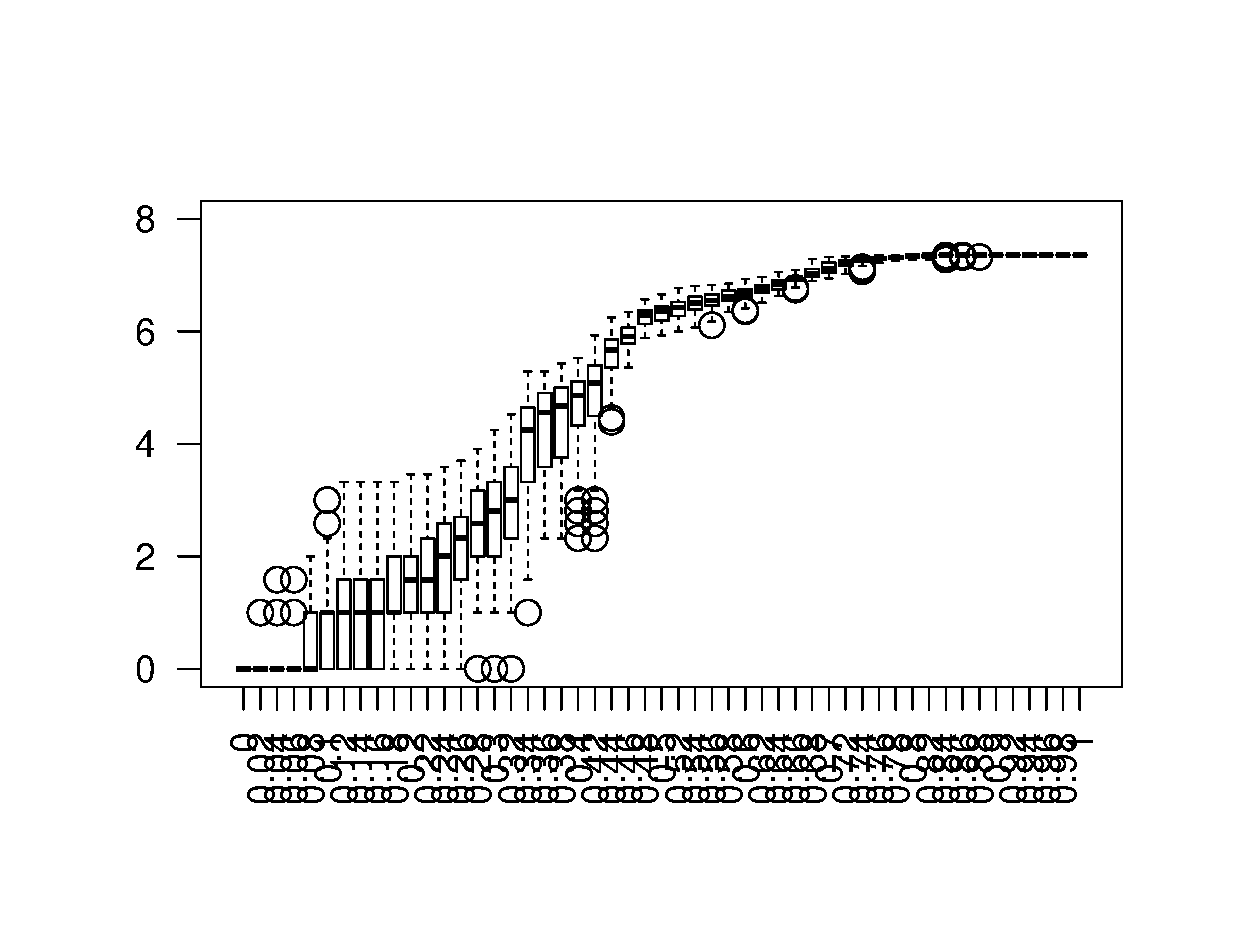
\includegraphics[width=7cm]{n08_full_small_emp.eps}

    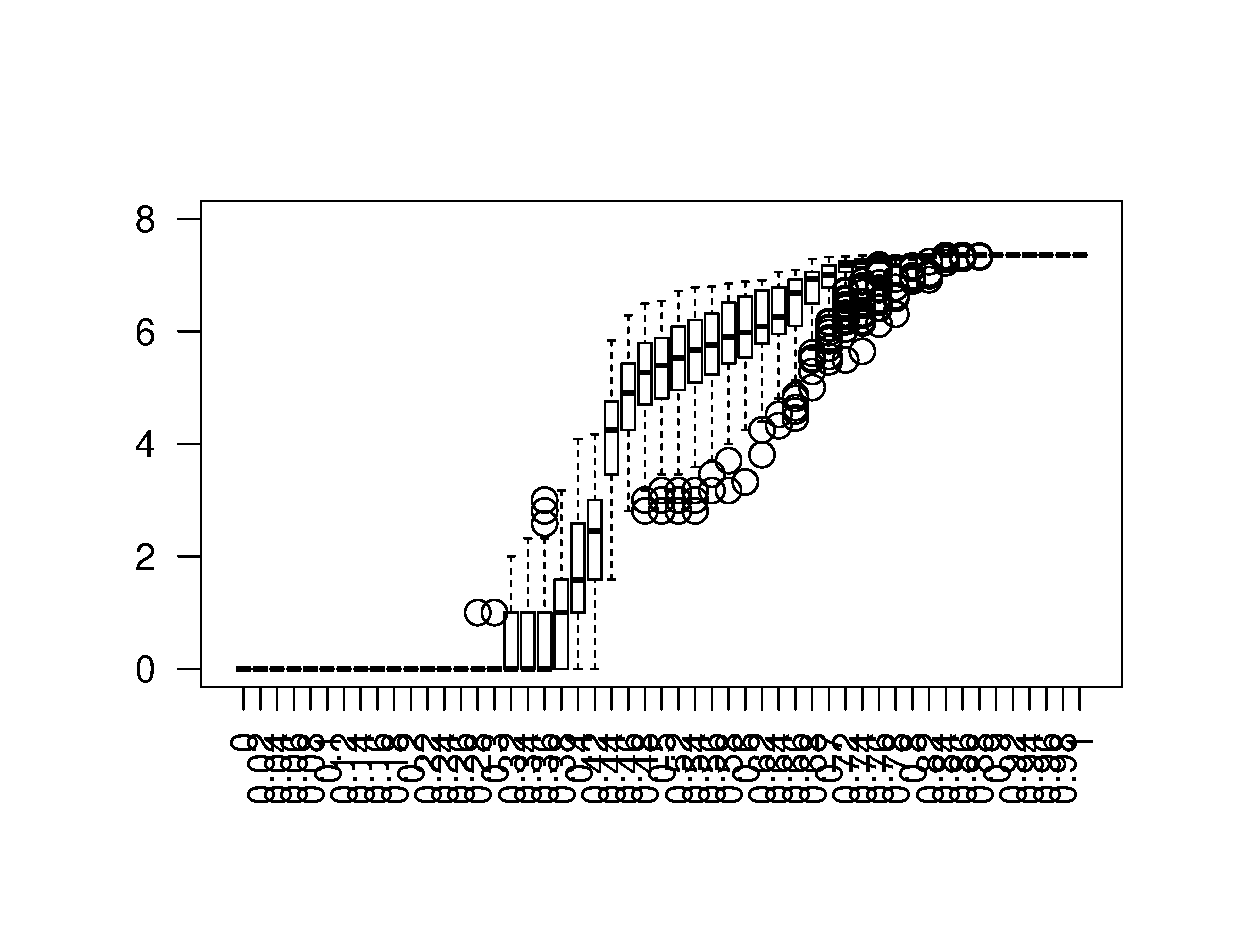
\includegraphics[width=7cm]{n08_full_small_empsust.eps}

  \end{center}

  \caption{Empowerment (top panel) and sustainable empowerment
    (bottom panel) as a function of $E$. Each boxplot summarises
    sustainability values for all initial states. The middle bar of
    a box shows the median, the box indicates the central quartiles,
    whiskers extend to the furthest point less than 1.5 times the
    interquartile range, and points outside this range are plotted
    individually.}
  \label{fig_empowermentprofiles}
\end{figure}

\dpnote{I believe axes will still be processed}

Empowerment and sustainable empowerment as a function of $E$ are shown
in Fig.~\ref{fig_empowermentprofiles}.

(to be completed from Old Discussion in appendix)


\begin{figure}

  \begin{center}

    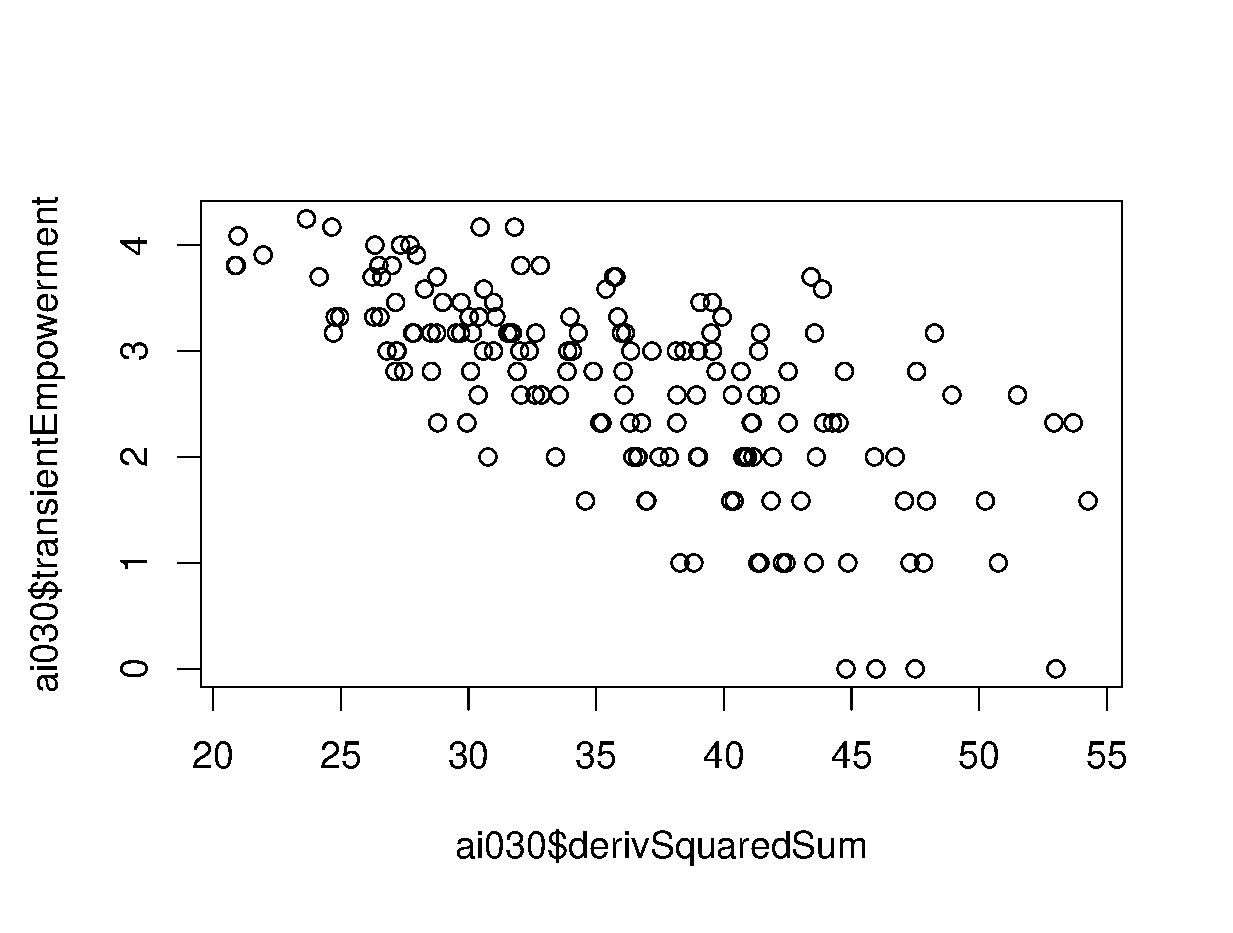
\includegraphics[width=7cm]{n08_full_small_corr_dss_emp_ai030.eps}

    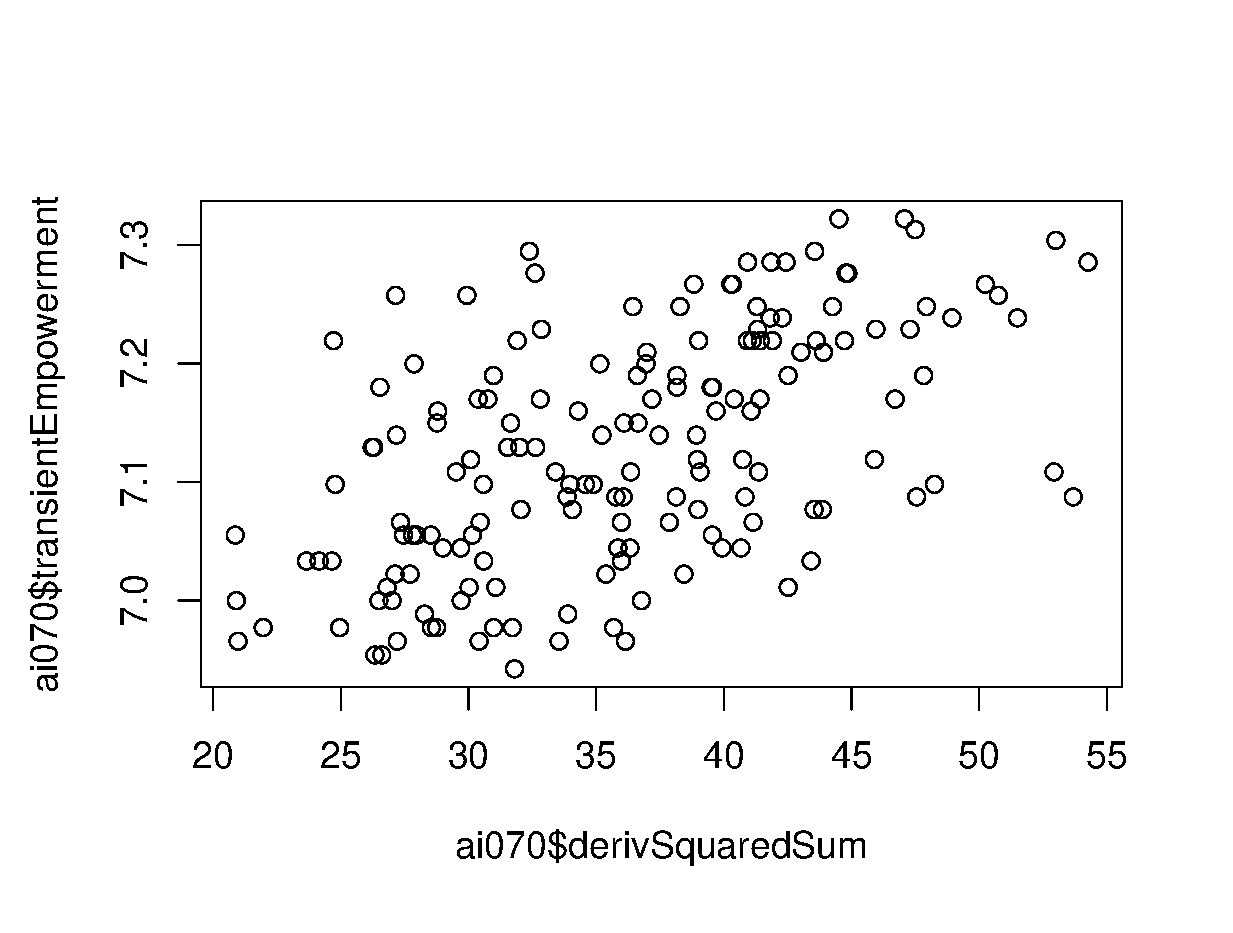
\includegraphics[width=7cm]{n08_full_small_corr_dss_emp_ai070.eps}

  \end{center}

  \caption{Scatterplot of the sum of derivative squares and
    empowerment at $E = 0.3$ (top) and $E = 0.7$ (bottom).}
  \label{fig_dssemp}

\end{figure}

Fig.~\ref{fig_dssemp} shows scatterplots of the sum of derivative
squares. At the smaller actuator range $E = 0.3$, empowerment
decreases as the sum of derivative square increases. At the larger
value $E = 0.7$, this trend reverses to a positive correlation.
\dpnote{This means?}


\begin{figure}

  \begin{center}

    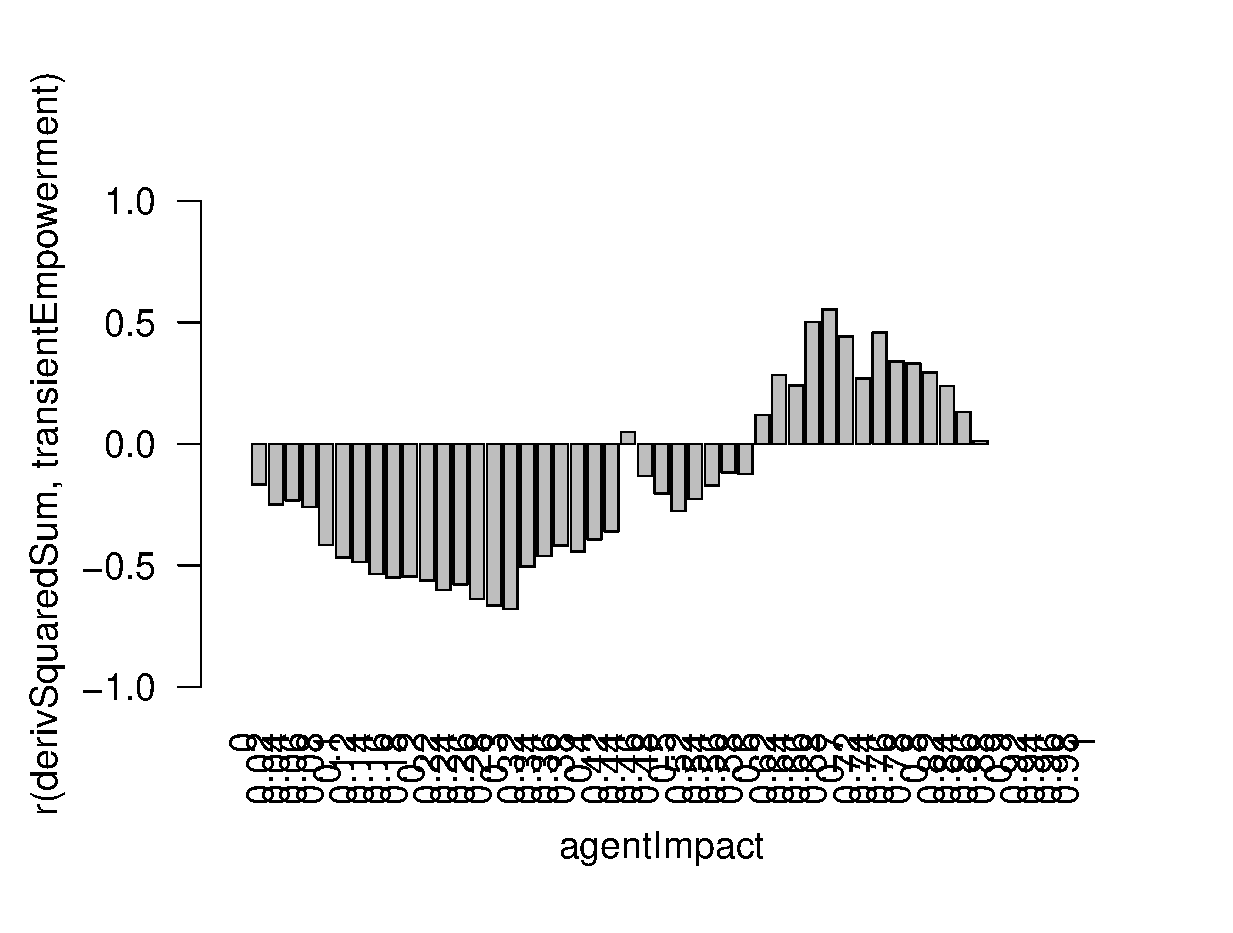
\includegraphics[width=7cm]{n08_full_small_corr_dss_emp.eps}

    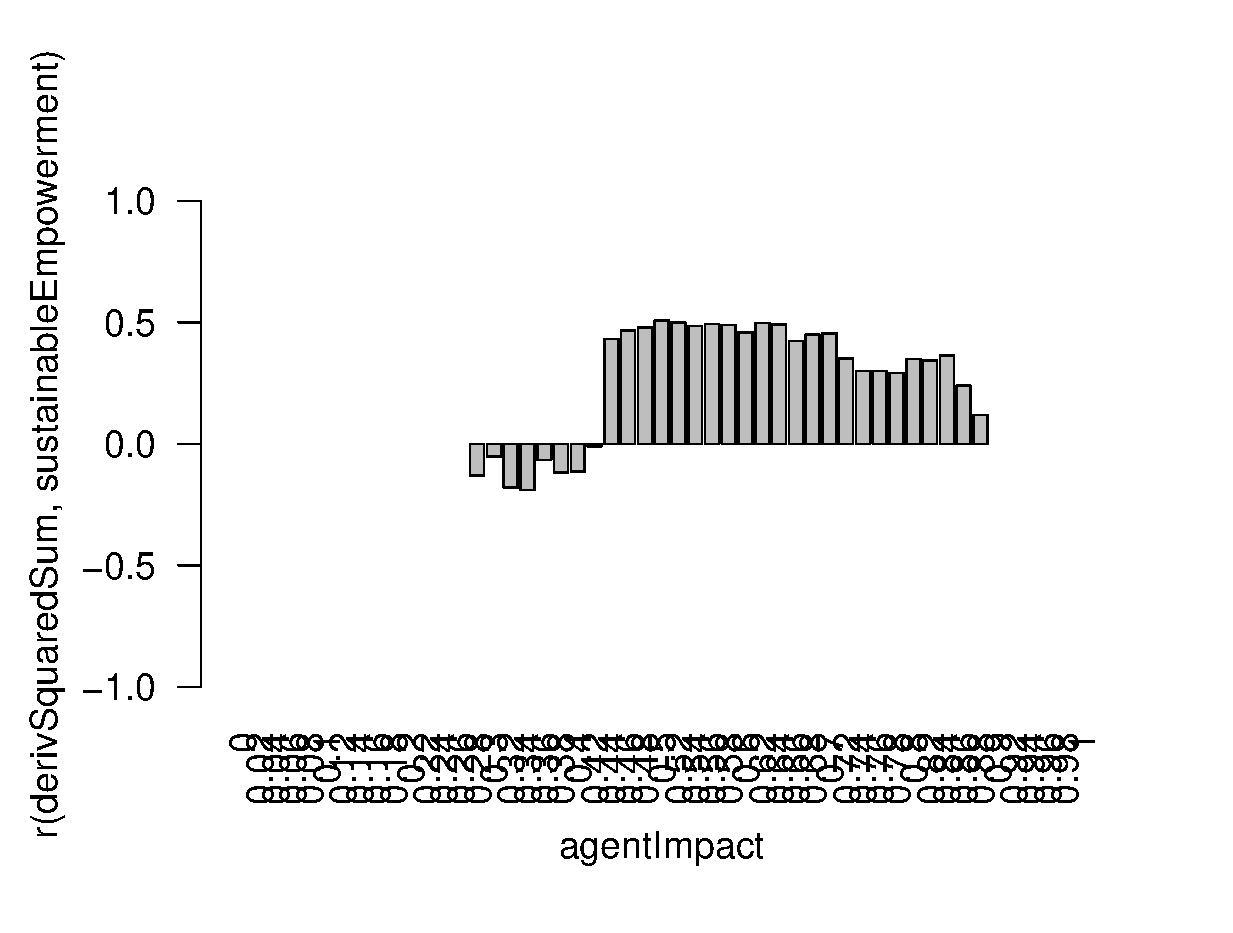
\includegraphics[width=7cm]{n08_full_small_corr_dss_empsust.eps}

  \end{center}

  \caption{Pearson correlation coefficients between the sum of derivative
    squares and empowerment (top) and between the sum of derivative
    squares and sustainable empowerment (bottom).}
  \label{fig_dssempcorr}

\end{figure}

Fig.~\ref{fig_dssempcorr} shows the Pearson correlation coefficients
between the sum of derivative squares and empowerment and sustainable
empowerment, respectively. \dpnote{And we see?}

The pattern of negative correlations at small values of $E$ and
positive correlations at larger values is corroborated. For
sustainable empowerment, positive correlations at larger values of $E$
are also found, while a negative correlation at small $E$ is largely
missing. \dpnote{This is an important observation because it shows
  that, once one only considers sustainable empowerment which takes
  into account reversibility, one concentrates on impact where the
  environment exhibits enough stability to be able counteract it (I
  assume this was more or less your argument)}



\section{Discussion and Outlook}

\textbf{to be updated and extended to discuss stability / correlation
  to sum of derivative squares}

% This deficiency has long been an impediment to public discourse
% \cite{Kim2001_plantbiodiversity}.

We have introduced systems comprised of coupled tipping elements
affected by an agent as a model to study sustainability and to
quantify it using the principled concept of empowerment
\cite{Salge2014_empowermentintro}, rooted in information theory
\cite{CoverThomas1991_informationtheory}. The cubic differential
equation systems which we use here capture essential aspects of
sustainability have been applied in sustainability research and
beyond, as reviewed e.g.\ by
\cite{Klose2019_interactingtippingelements}. By explicitly including
an agent, our system opens up opportunities to model sustainability as
a property that emerges as some kind of external actor interacts with
the system. This allows for a more precise characterisation and
formalisation of sustainability under active and intention-driven
stressors (one main use of empowerment is the modeling of
intention-carrying intrinsically motivated agents). This separates
this work from investigating more general questions of system, such as
ecosystem stability.

Our plans to further develop this approach include studying the
effects of providing the agent with different actuation channels. An
alternative to allowing the agent to impact all elements equally is to
restrict the agent to impact only one or few elements directly. In
this scenario, high levels of empowerment result only if the agent is
able to affect a large number of elements indirectly via their
coupling. We therefore anticipate that stronger coupling will
increase, rather than decrease, empowerment. It will be interesting to
investigate whether susceptibility to ``domino effects'' between
elements can be characterised in this way, and specifically systems in
which only one or few elements can cause  downstream elements to tip, as
described by \cite{Brummitt2015_coupledcatastrophes}. \dpnote{Did I
  capture that correctly, or am I misrepresenting?}

Empowerment in its general form considers an agent to receive signals
from the environment, and to send signals to the environment through
its actuators. Both sensors and actuators can be affected by noise. As
humankind, we have only partial and noisy data from our environment,
and our control over our action at a population or society level is
imperfect as well. Therefore, it is important to understand the impact
of these imperfections on sustainability.


% TODO discuss asymmetry
% Shifting the offset c in a tipping unit permits producing a
% hysteresis which makes it easier (for the agent) to "tip" the system
% into the other stable state, while the reverse operation becomes
% more difficult.

It is interesting to note that the offset $c$ produces a hysteresis
which makes it easier for the agent to tip the system in one direction
(from $x_{-}$ to $x_{+}$ if $c > 0$) while the reverse operation
becomes more difficult. This enables applying the concept of
sustainable empowerment, which we introduced in
\cite{Kim2009_sustainability}, to systems of coupled tipping elements
as well. \dpnote{what's the difference to what we do now?}

Finally, a strength of our model is that it allows efficient
computation of fixed point as well as integrating differential
equations to produce time series. This opens perspectives to
investigate the potential to use time series for
characterising and quantifying sustainability, for instance as a tool to
identify risks and early warning signs of breakdowns in sustainability
or to identify elements that are especially relevant to maintaining
sustainability.




% From perspective for the work presented here include 

%  as minimalistic ALife systems
% to model essential aspects of sustainability in the context of an
% agent trying to maintain and manipulate an ecosystem. We have shown
% the essential properties \ref{hinz und kunz}, and demonstrated that
% this \ref{hurzt und schnurzt}, showing that the system can serve as a
% proof-of-concept framework to study the effect of reversible,
% sustainable management by an agent vs.\ its opposite.

%% However, they provide no inherent way of distinguishing between
%% sustainability and stability. In this paper we use them as a model of
%% an environment which interacts with an agent. This allows us to
%% characterise states that can be reached (and stabilised) by the
%% agent's actuators as candidates for sustainable states.

% perspectives on introducing noise?
% discuss interpretative scenarios, e.g. some "actuation" may benefit
% the agent and add to its ability whereas others may be "cost" --
% e.g. emitting more carbon may allow more Haber-Bosch nitrogen
% fixation...? but adding carbon capture may diminish / be a cost...?

% \section{Preliminary Results}

% \cleardoublepage

% \includegraphics[width=6cm]{coupledtippingdemo_x01.eps}

% \vspace{1cm}

% \includegraphics[width=6cm]{coupledtippingdemo_x02.eps}

% \vspace{1cm}

% \includegraphics[width=6cm]{coupledtippingdemo_x03.eps}

% \vspace{1cm}

% \includegraphics[width=6cm]{coupledtippingdemo_x04.eps}

% \vspace{1cm}

% \includegraphics[width=6cm]{coupledtippingdemo_x05.eps}

% \vspace{1cm}

% \includegraphics[width=6cm]{coupledtippingdemo_x06.eps}

% \vspace{1cm}

% \includegraphics[width=6cm]{coupledtippingdemo_x07.eps}

% \vspace{1cm}

% \includegraphics[width=6cm]{coupledtippingdemo_x08.eps}

% \vspace{1cm}

% \includegraphics[width=6cm]{coupledtippingdemo_x09.eps}

% \vspace{1cm}

% \includegraphics[width=6cm]{coupledtippingdemo_x10.eps}


% \begin{table}[htbp]
% \caption{Table Type Styles}
% \begin{center}
% \begin{tabular}{|c|c|c|c|}
% \hline
% \textbf{Table}&\multicolumn{3}{|c|}{\textbf{Table Column Head}} \\
% \cline{2-4} 
% \textbf{Head} & \textbf{\textit{Table column subhead}}& \textbf{\textit{Subhead}}& \textbf{\textit{Subhead}} \\
% \hline
% copy& More table copy$^{\mathrm{a}}$& &  \\
% \hline
% \multicolumn{4}{l}{$^{\mathrm{a}}$Sample of a Table footnote.}
% \end{tabular}
% \label{tab1}
% \end{center}
% \end{table}

% \begin{figure}[htbp]
% \centerline{\includegraphics{fig1.png}}
% \caption{Example of a figure caption.}
% \label{fig}
% \end{figure}


\bibliographystyle{IEEEtran}
\bibliography{bioinfo}

\cleardoublepage

\appendix

\subsection{Complete Set of Plots}


\subsubsection{small interactions, full connectivity}

\rule{0pt}{0pt}

\centerline{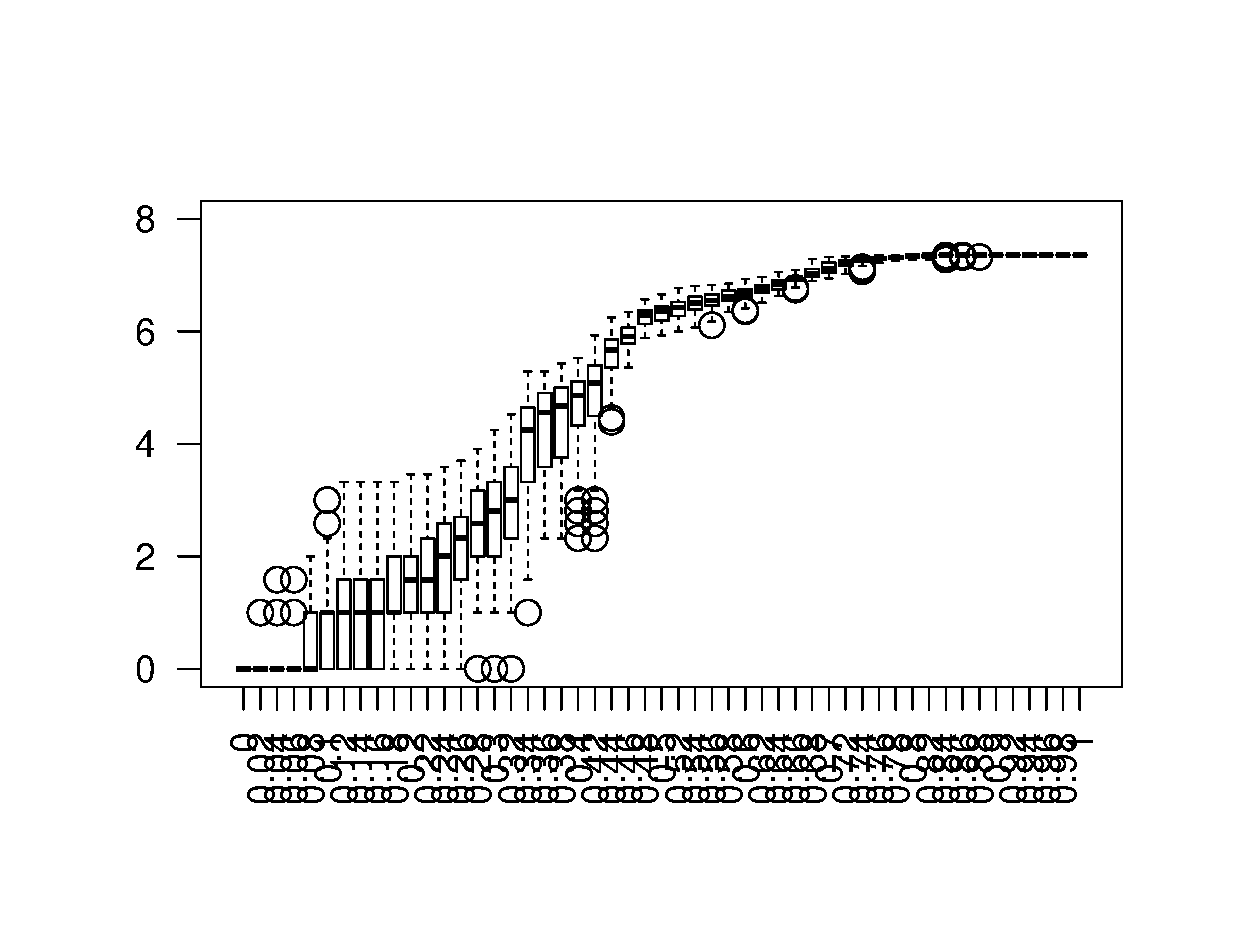
\includegraphics[width=7cm]{n08_full_small_emp.eps}}

\centerline{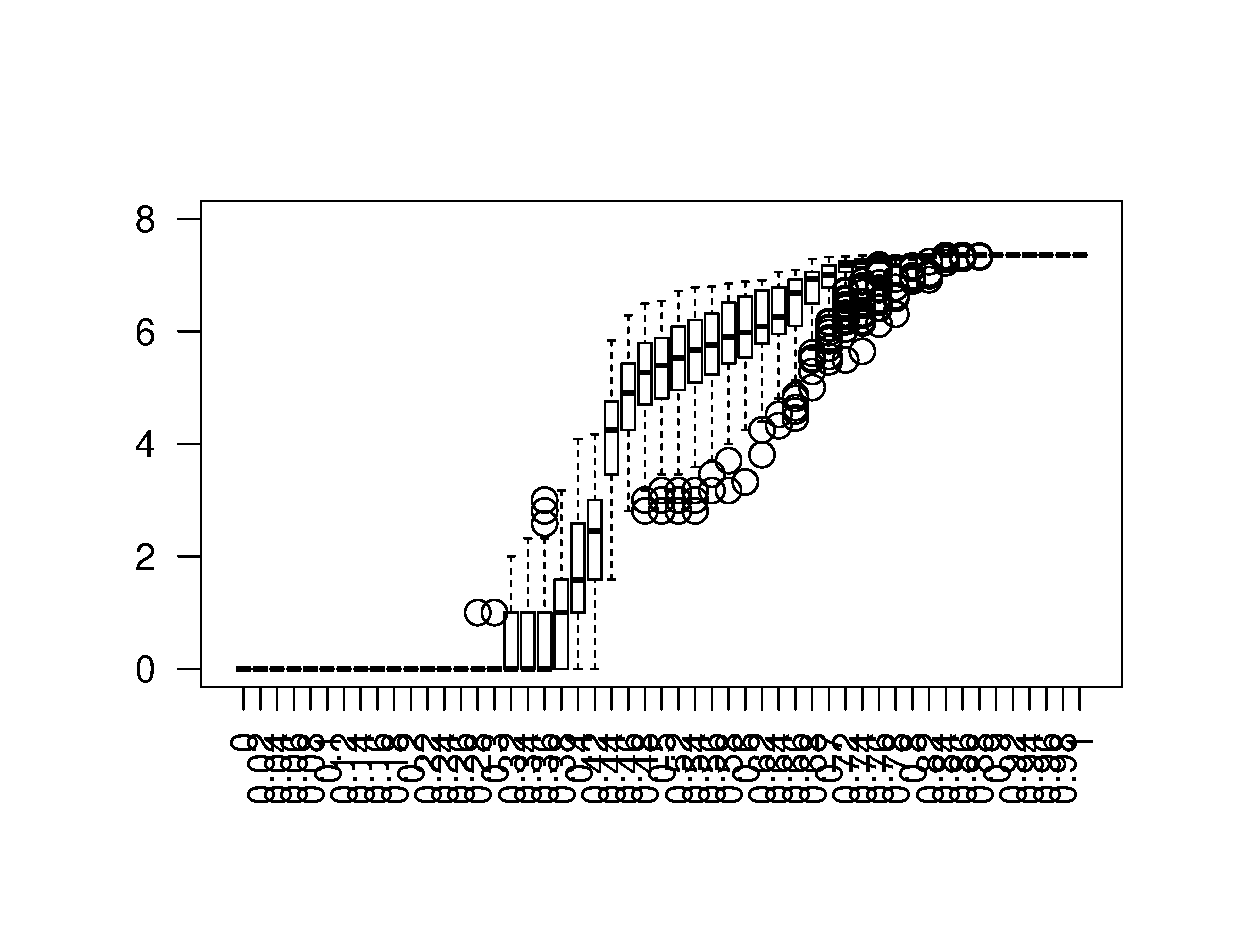
\includegraphics[width=7cm]{n08_full_small_empsust.eps}}

\centerline{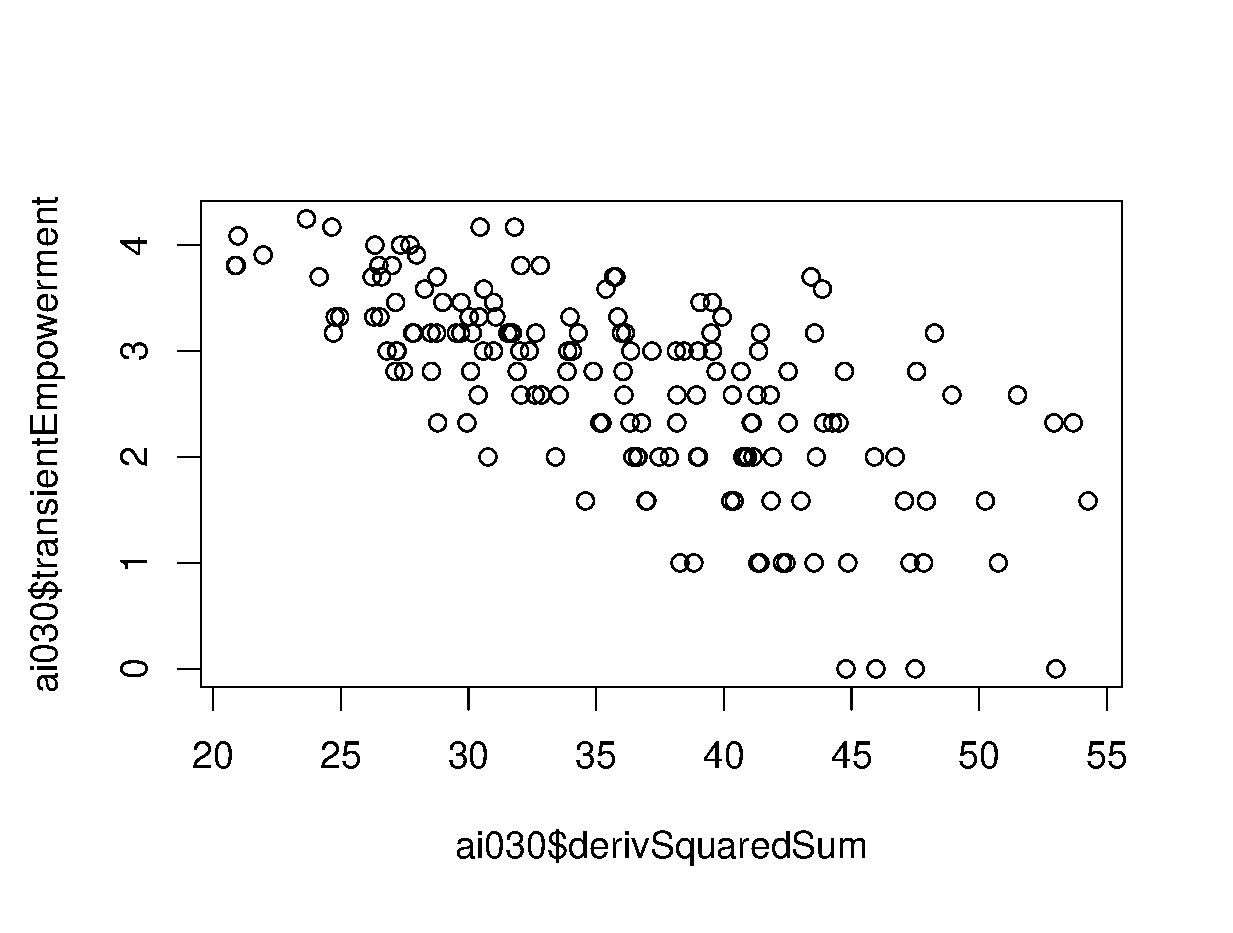
\includegraphics[width=7cm]{n08_full_small_corr_dss_emp_ai030.eps}}

\centerline{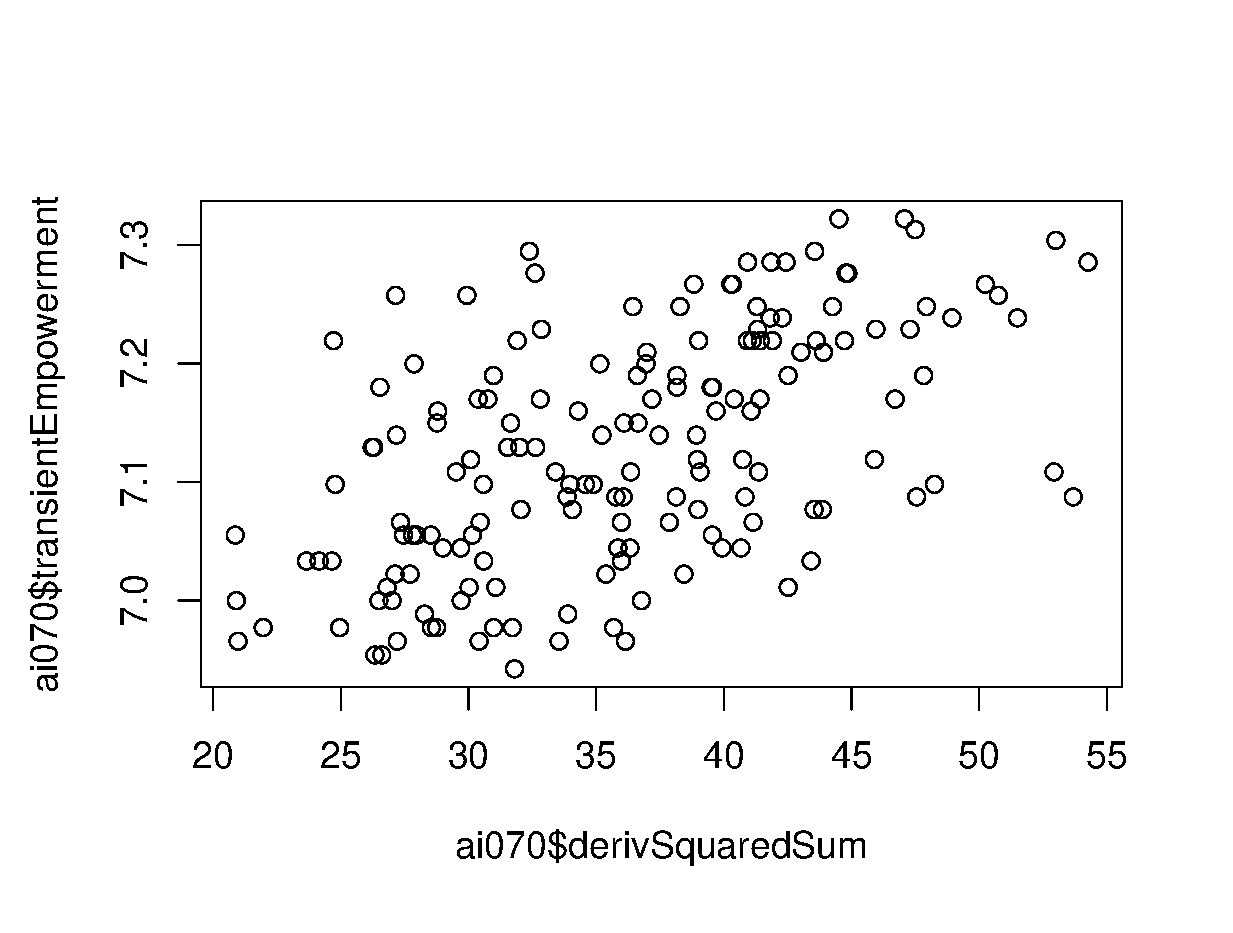
\includegraphics[width=7cm]{n08_full_small_corr_dss_emp_ai070.eps}}

\centerline{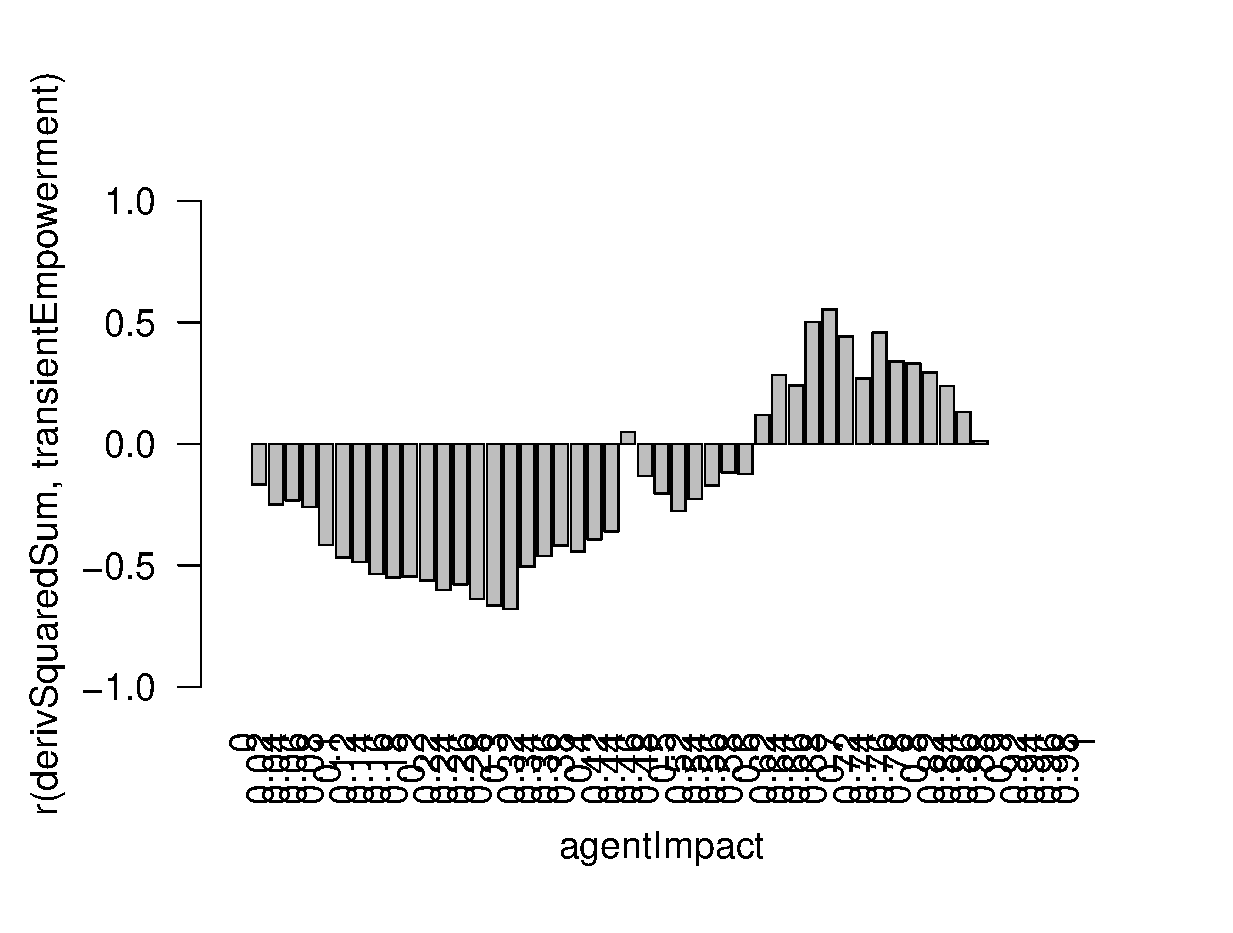
\includegraphics[width=7cm]{n08_full_small_corr_dss_emp.eps}}

\centerline{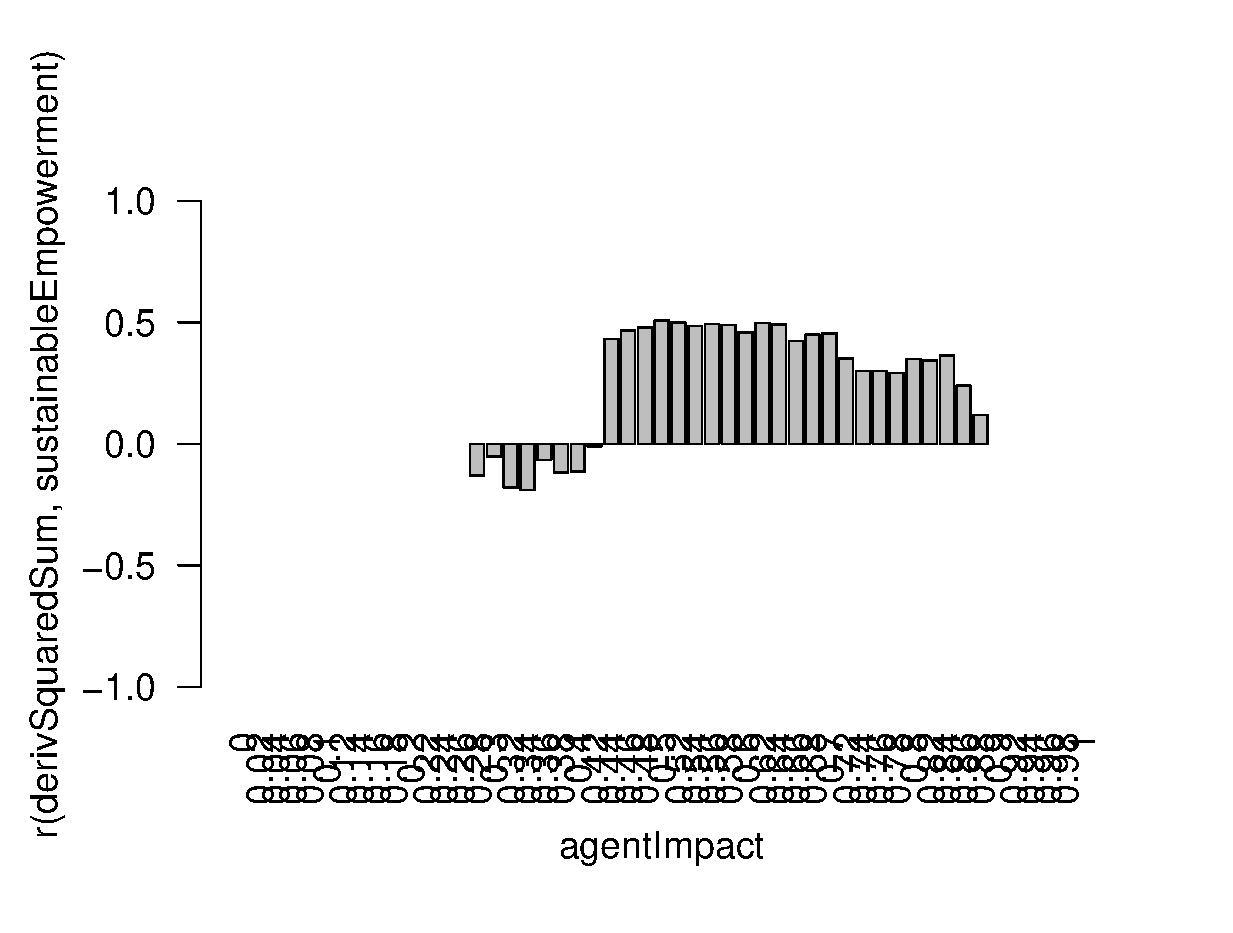
\includegraphics[width=7cm]{n08_full_small_corr_dss_empsust.eps}}


\pagebreak


\subsubsection{large interactions, full connectivity}

\rule{0pt}{0pt}

\centerline{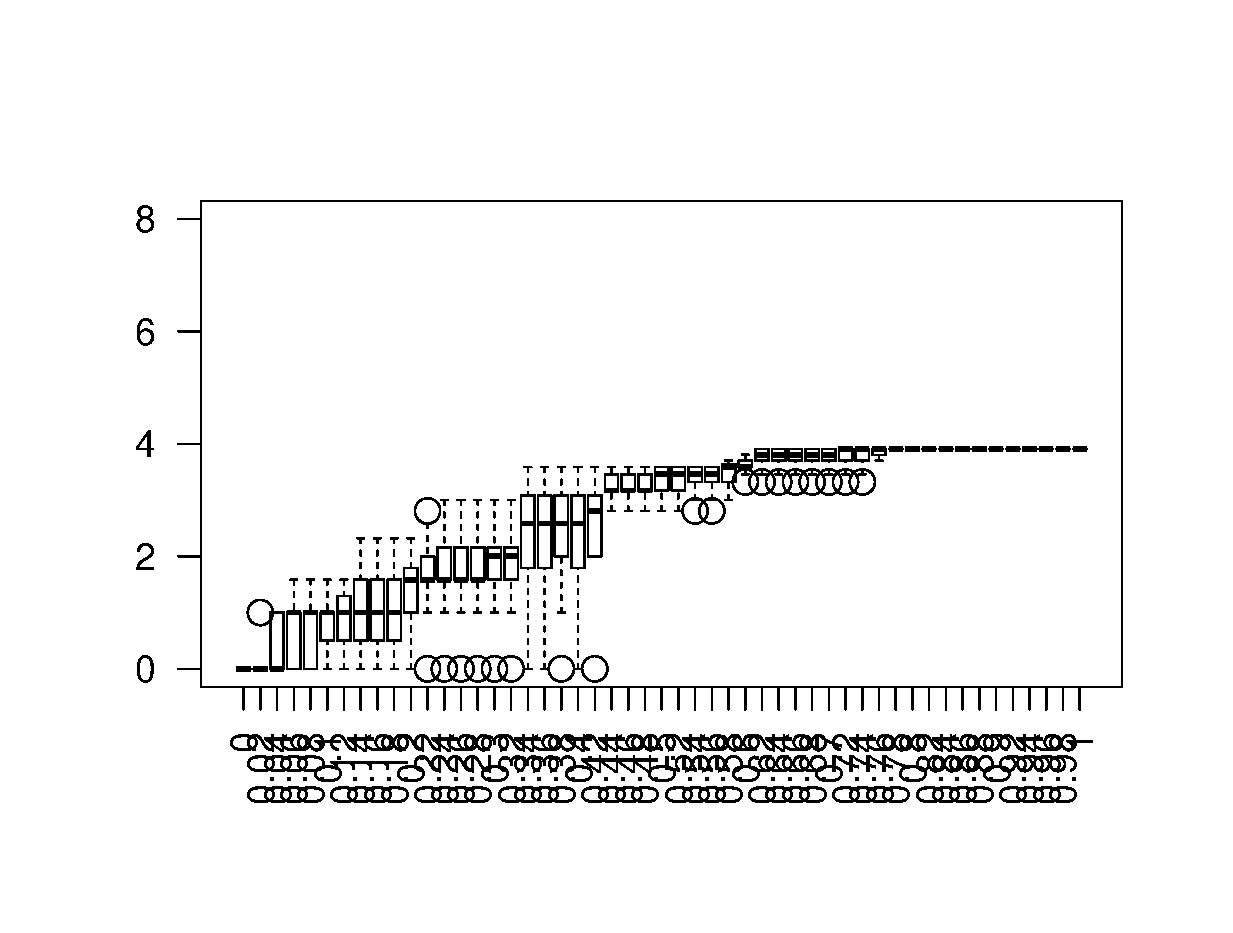
\includegraphics[width=7cm]{n08_full_large_emp.eps}}

\centerline{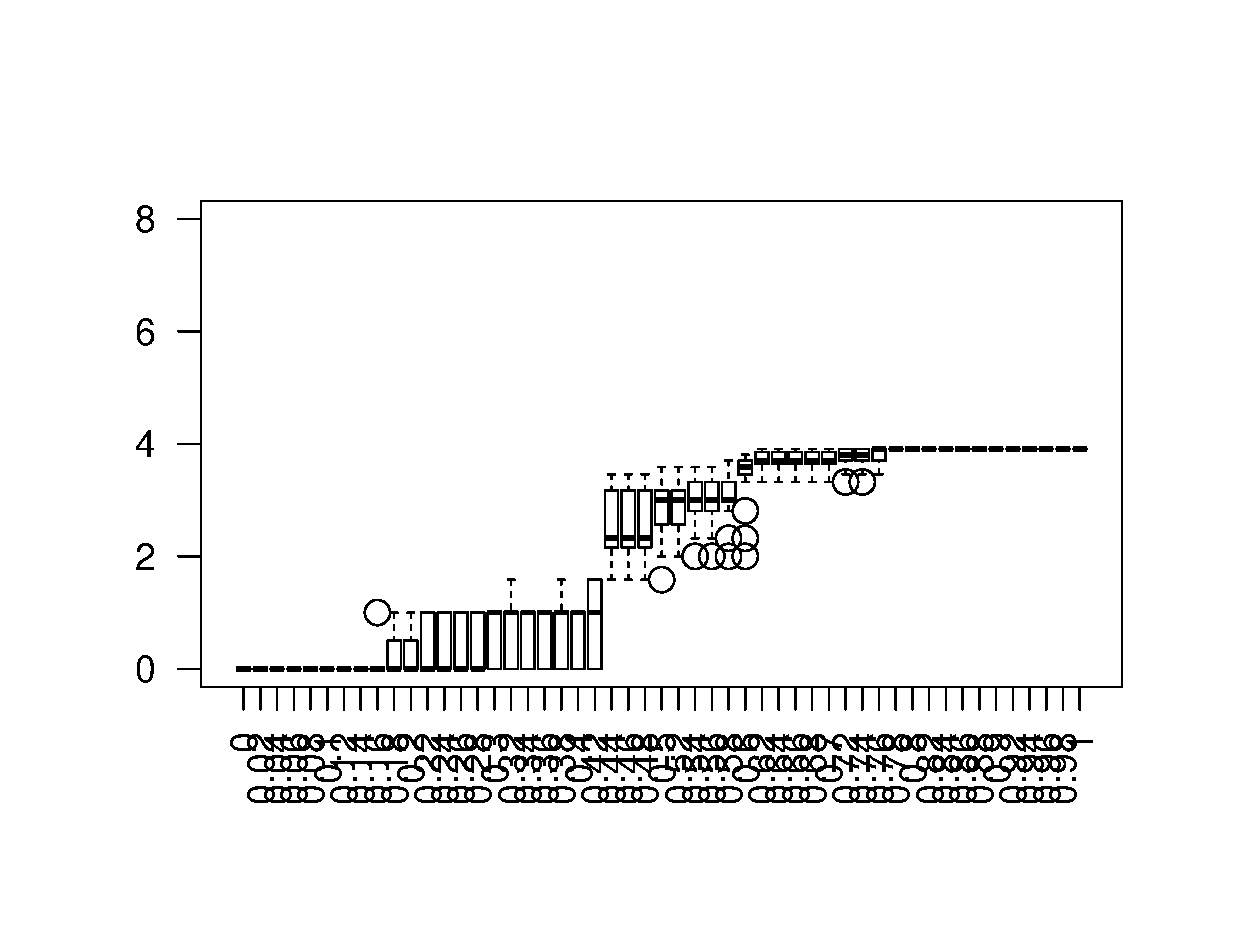
\includegraphics[width=7cm]{n08_full_large_empsust.eps}}

\centerline{\includegraphics[width=7cm]{n08_full_large_corr_dss_emp_ai030.eps}}

\centerline{\includegraphics[width=7cm]{n08_full_large_corr_dss_emp_ai070.eps}}

\centerline{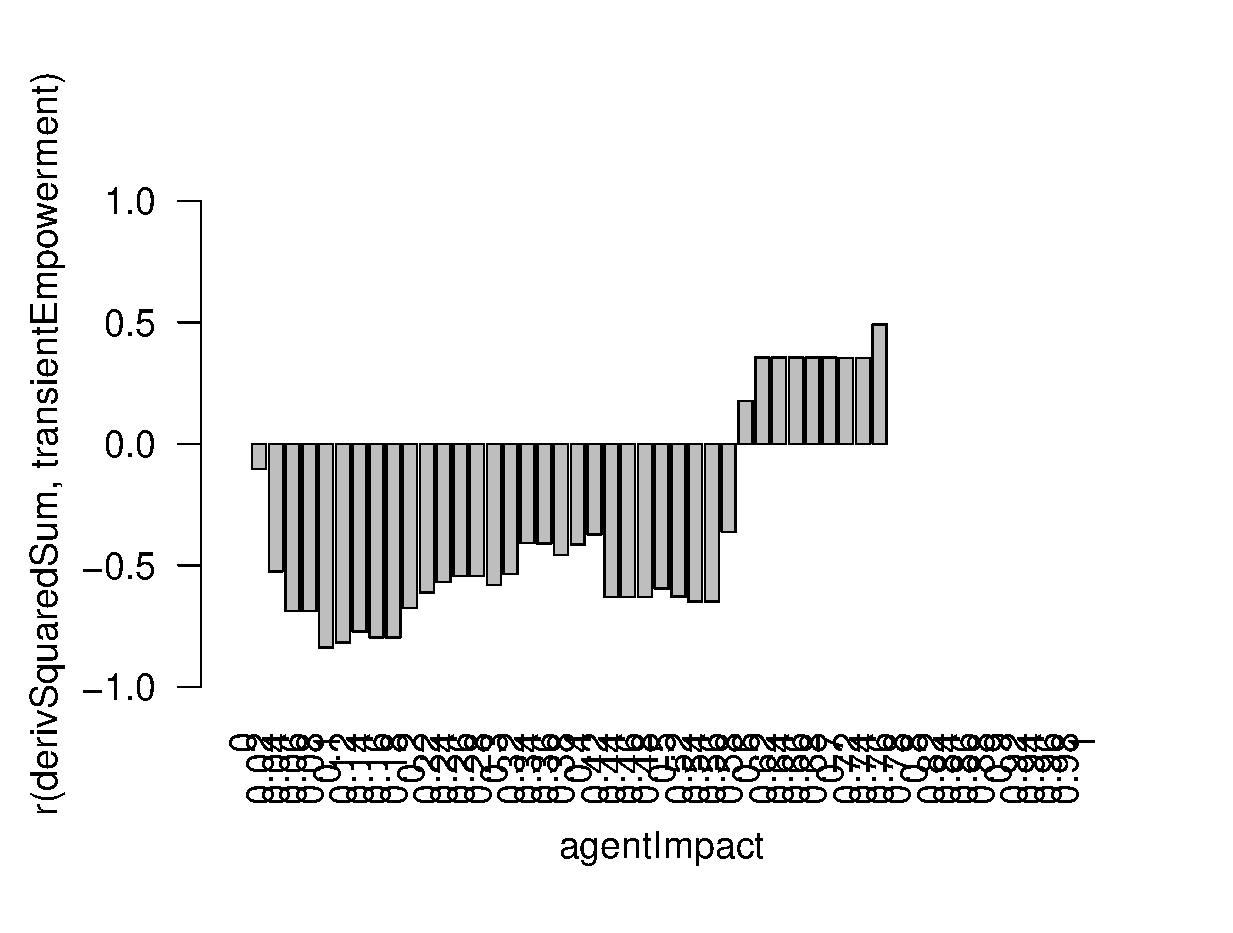
\includegraphics[width=7cm]{n08_full_large_corr_dss_emp.eps}}

\centerline{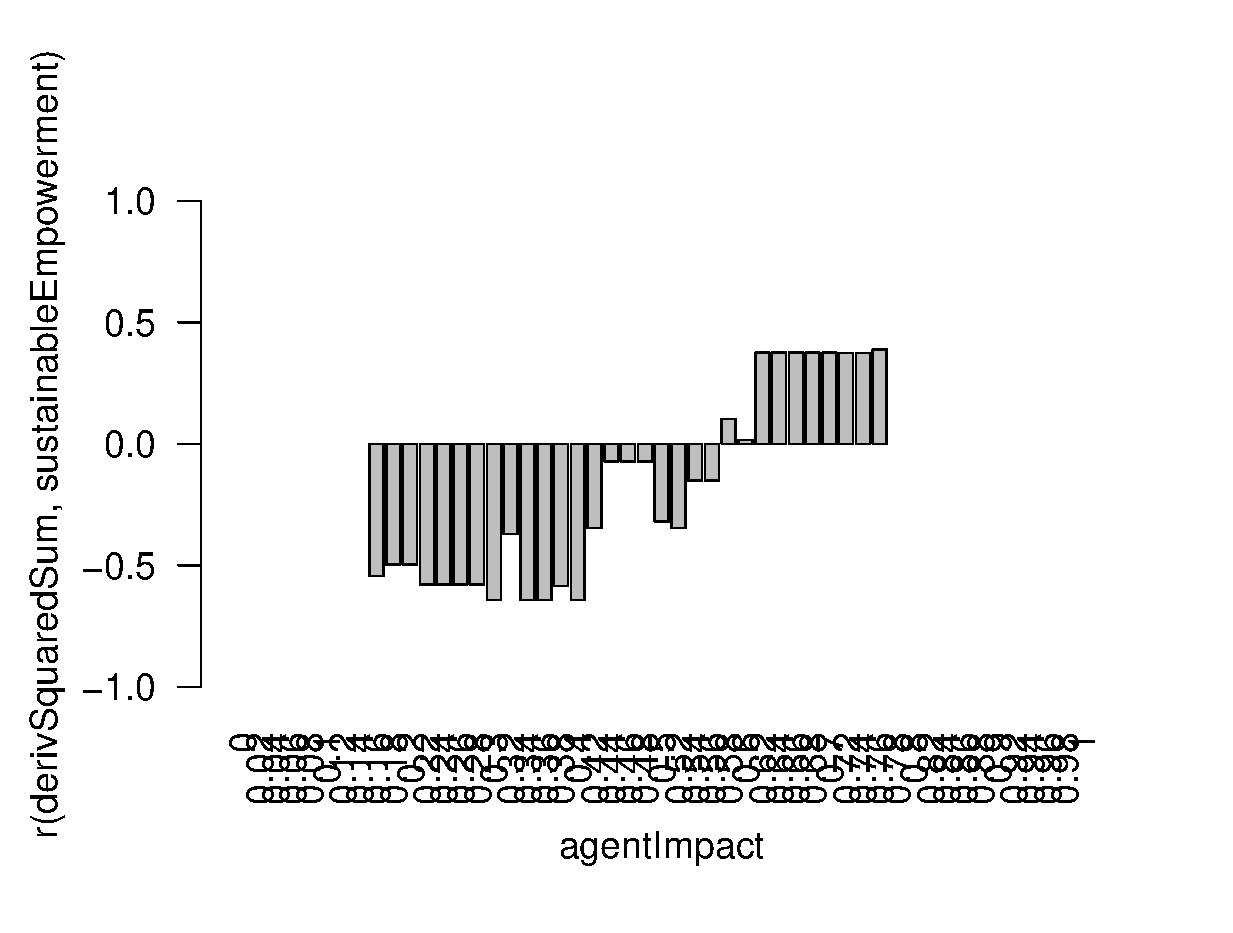
\includegraphics[width=7cm]{n08_full_large_corr_dss_empsust.eps}}


\pagebreak


\subsubsection{small interactions, chain connectivity}

\rule{0pt}{0pt}

\centerline{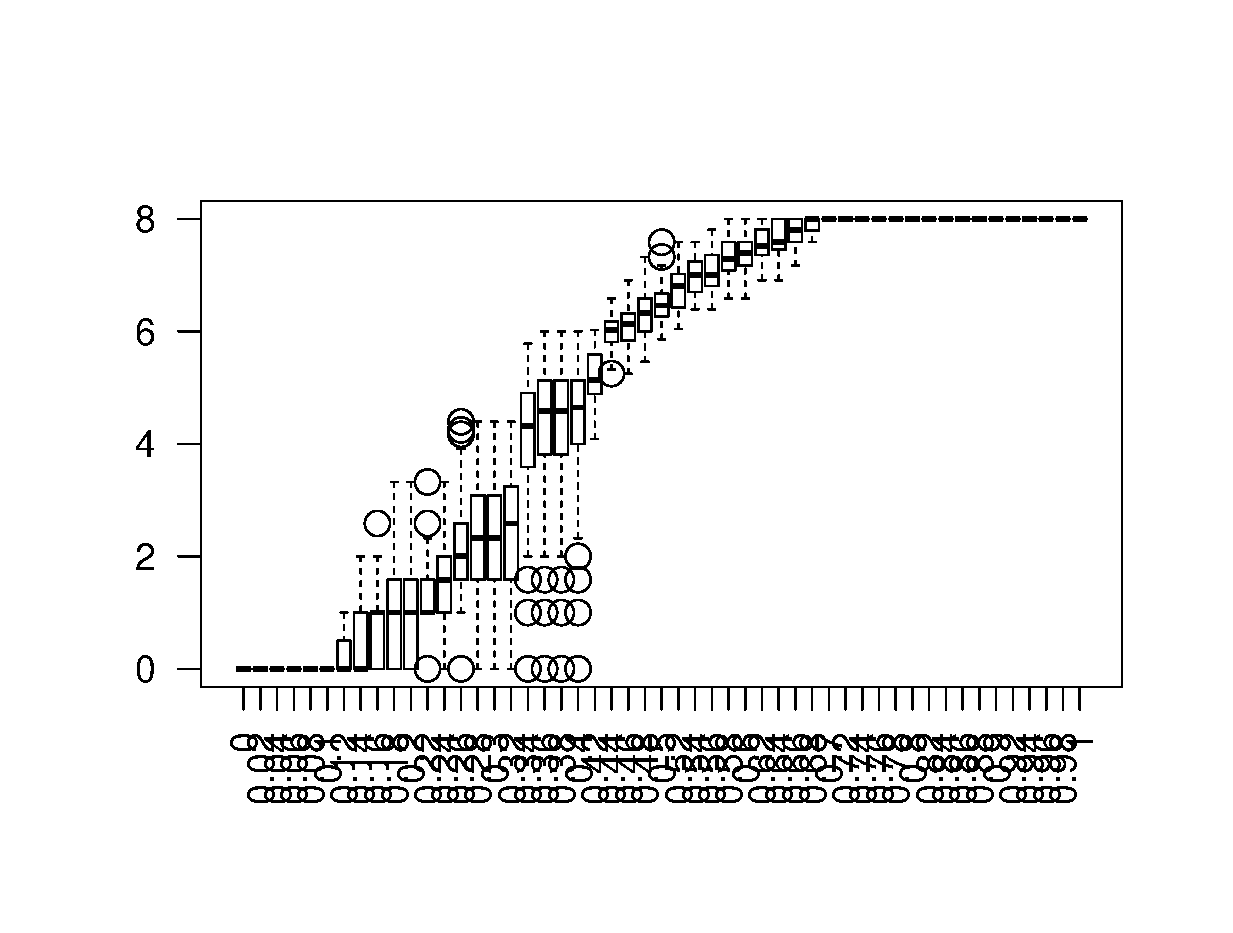
\includegraphics[width=7cm]{n08_chain_small_emp.eps}}

\centerline{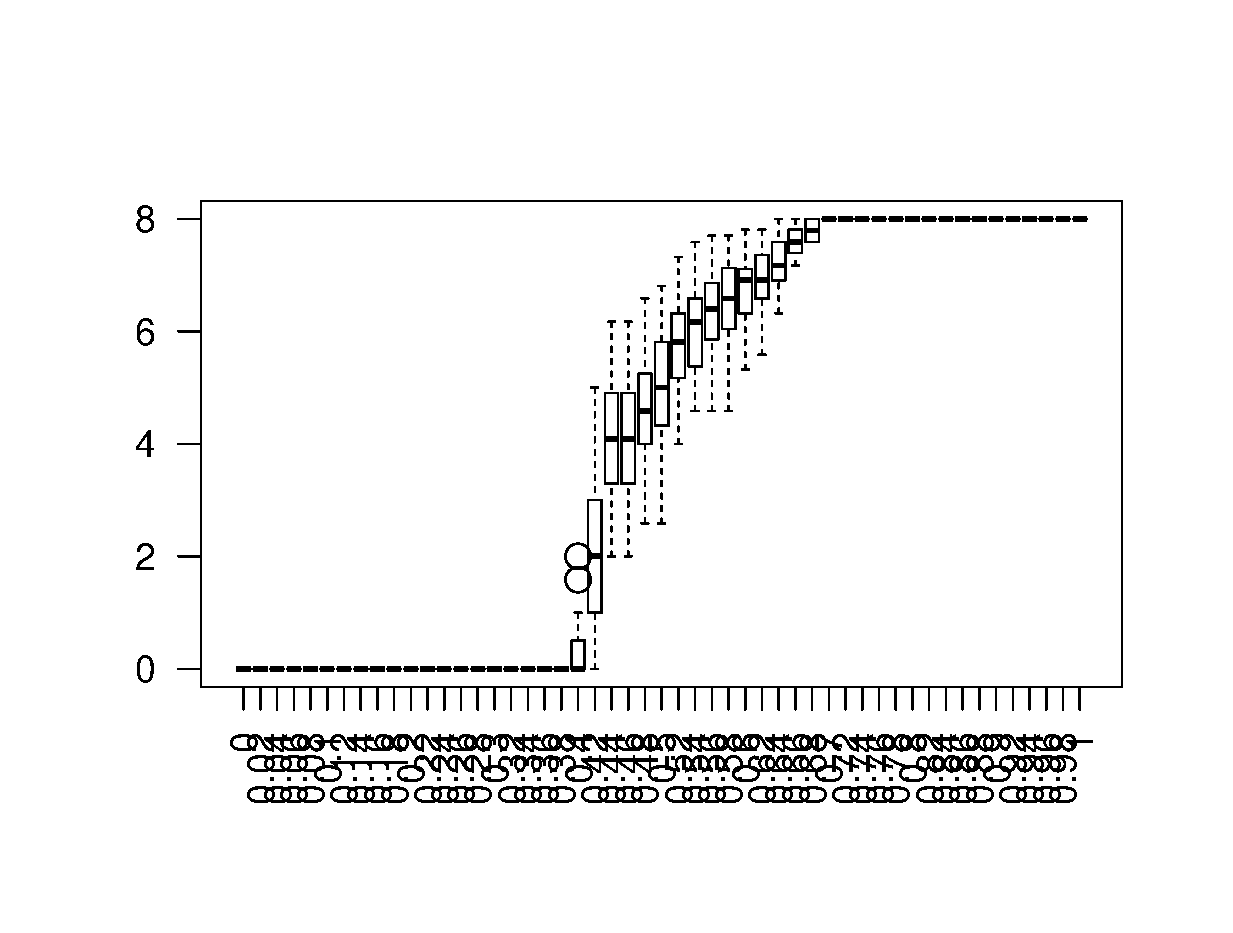
\includegraphics[width=7cm]{n08_chain_small_empsust.eps}}

\centerline{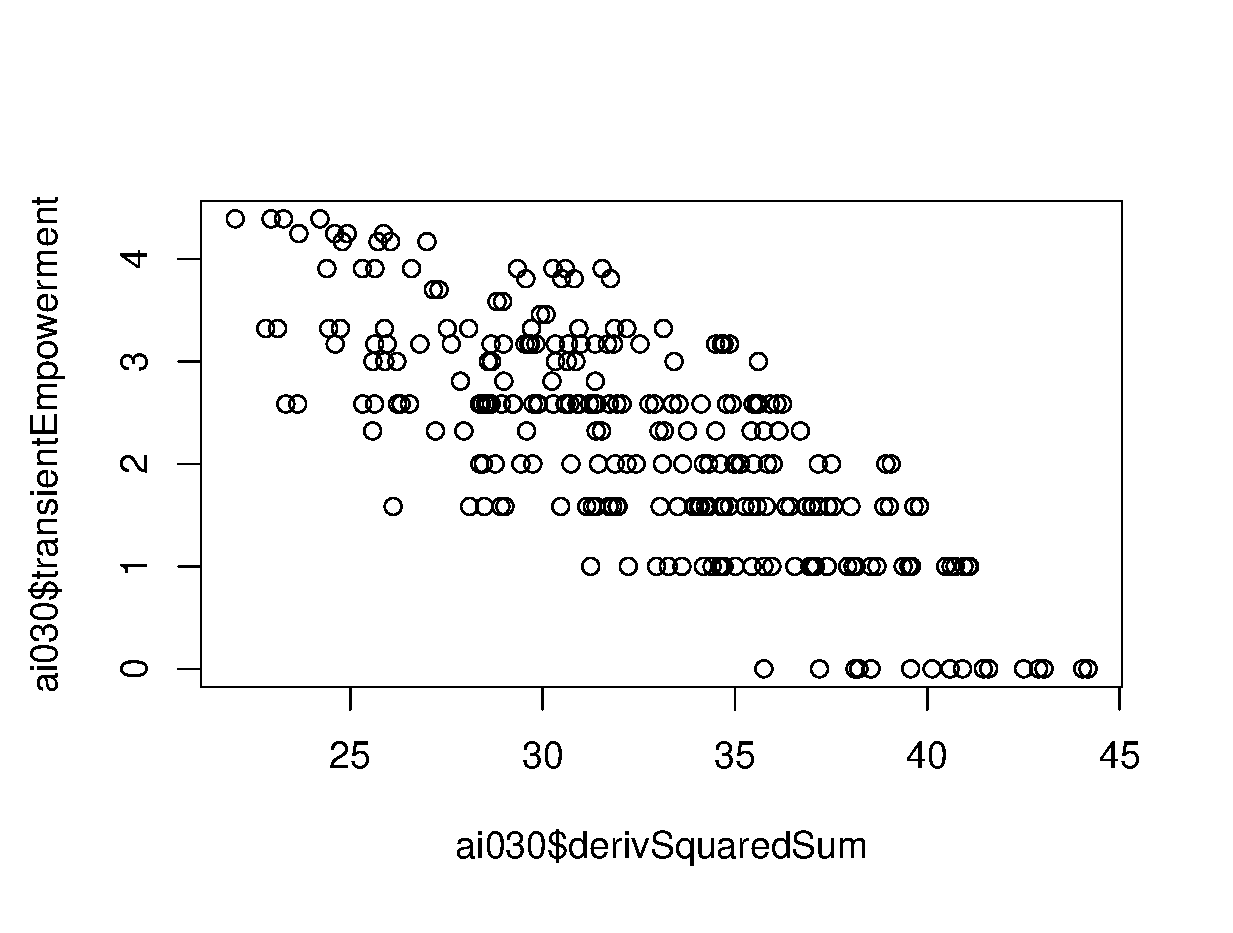
\includegraphics[width=7cm]{n08_chain_small_corr_dss_emp_ai030.eps}}

\centerline{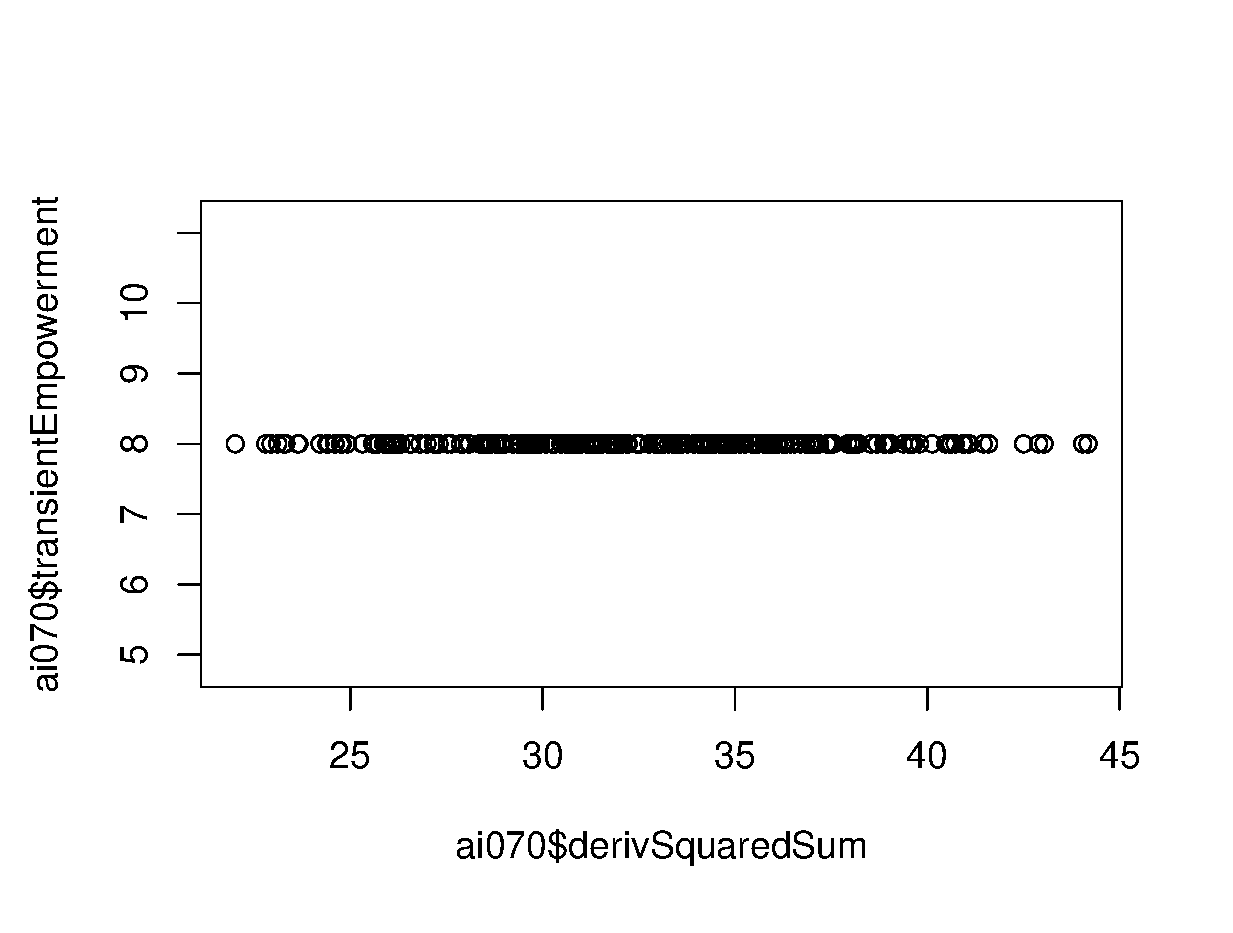
\includegraphics[width=7cm]{n08_chain_small_corr_dss_emp_ai070.eps}}

\centerline{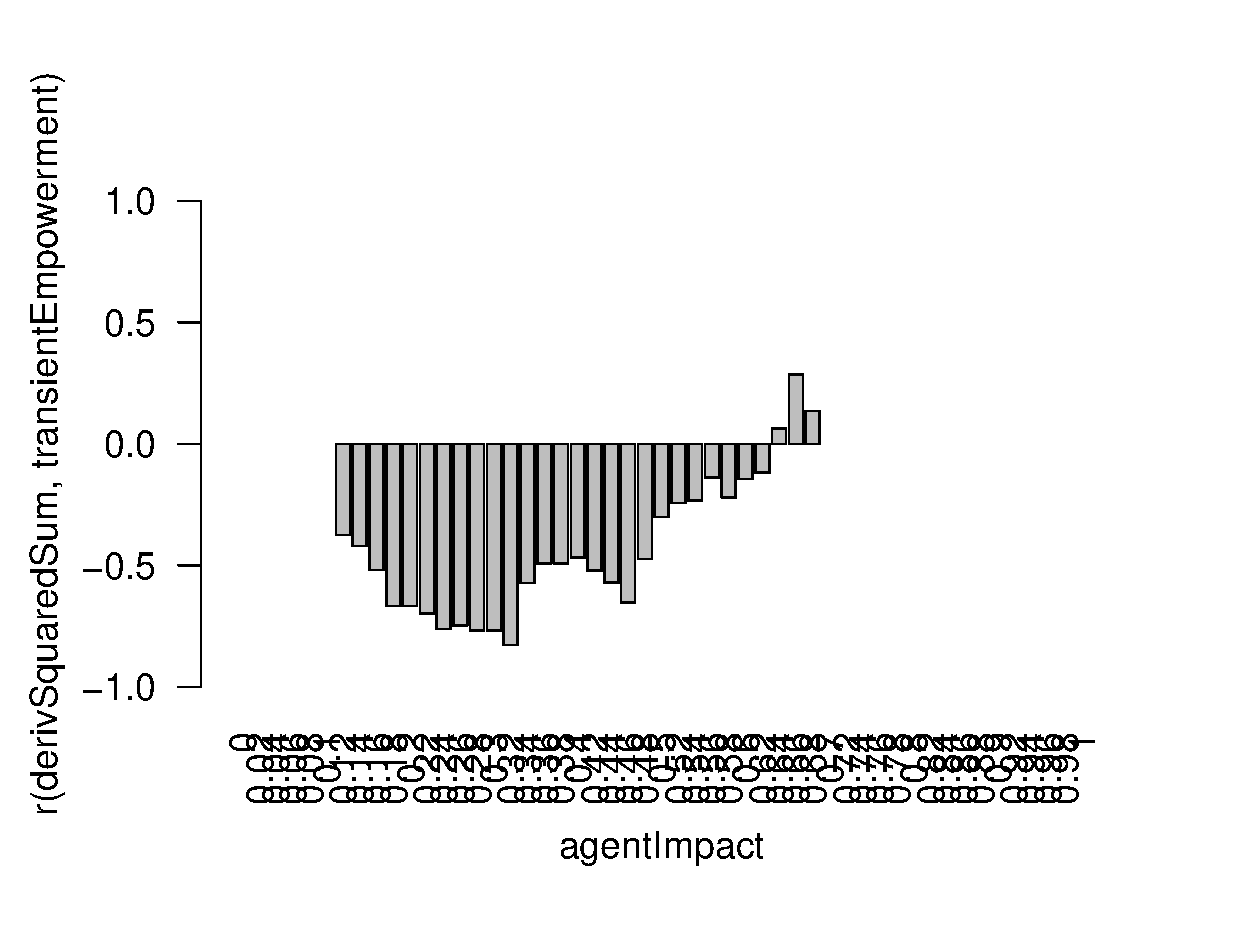
\includegraphics[width=7cm]{n08_chain_small_corr_dss_emp.eps}}

\centerline{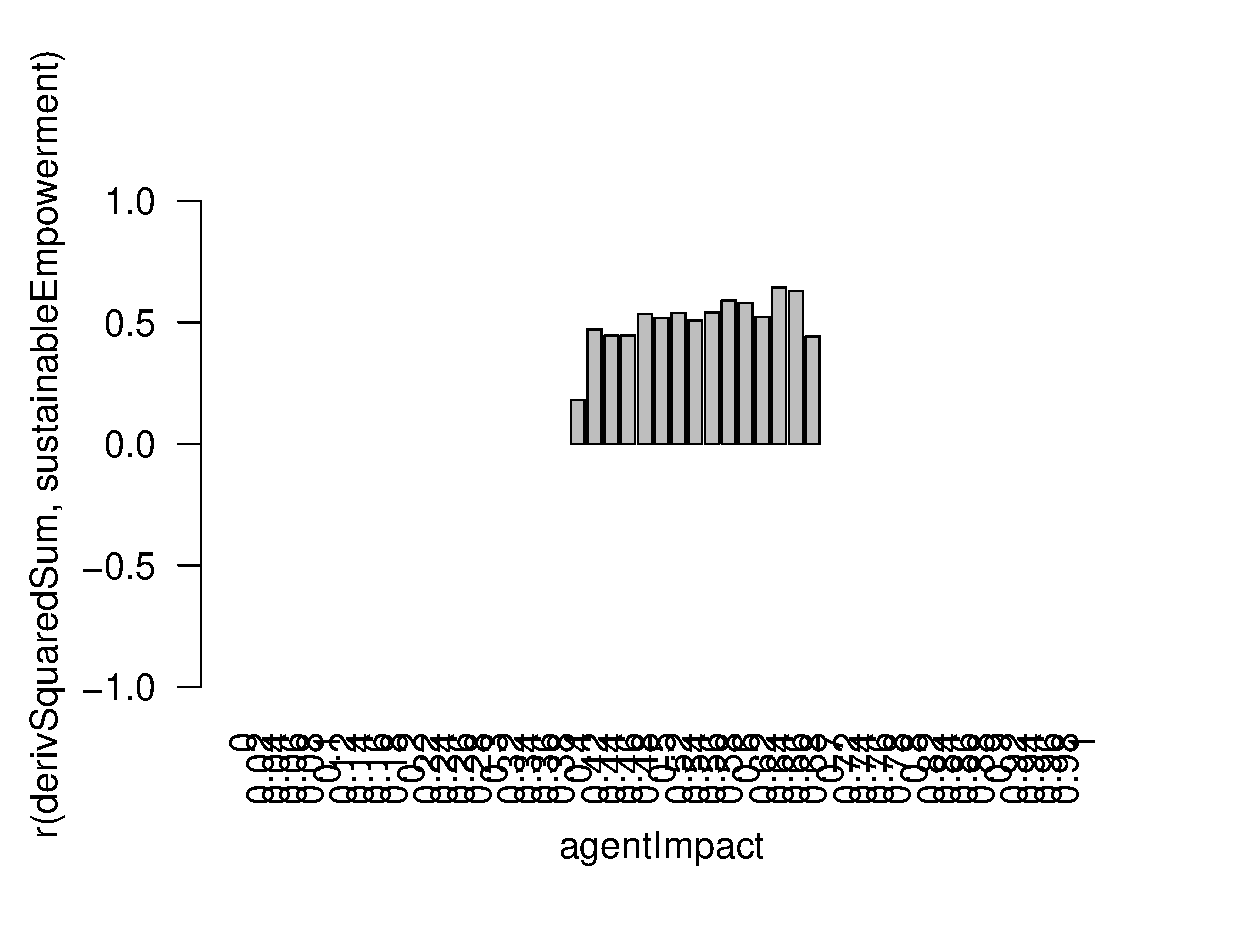
\includegraphics[width=7cm]{n08_chain_small_corr_dss_empsust.eps}}


\pagebreak


\subsubsection{large interactions, chain connectivity}

\rule{0pt}{0pt}

\centerline{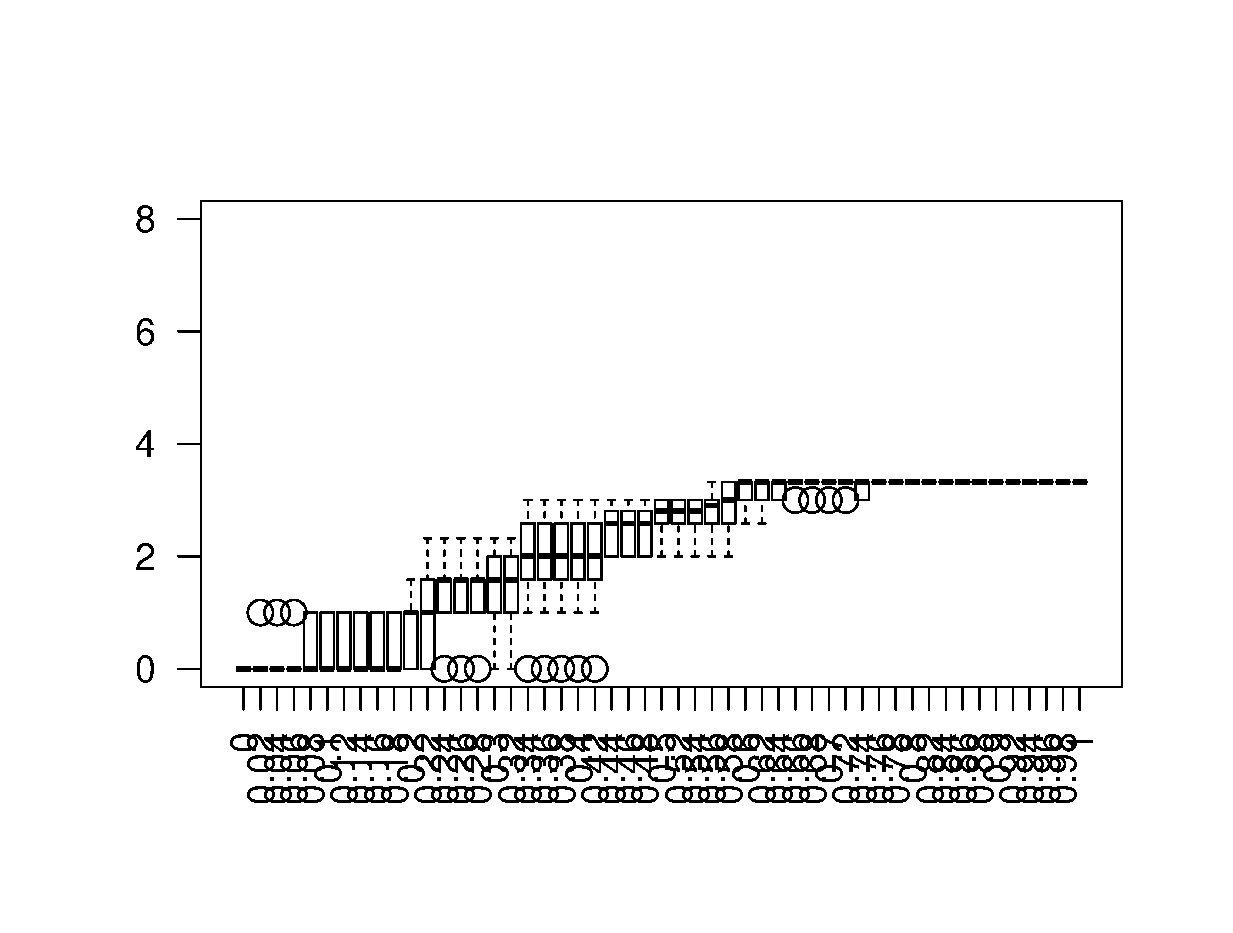
\includegraphics[width=7cm]{n08_chain_large_emp.eps}}

\centerline{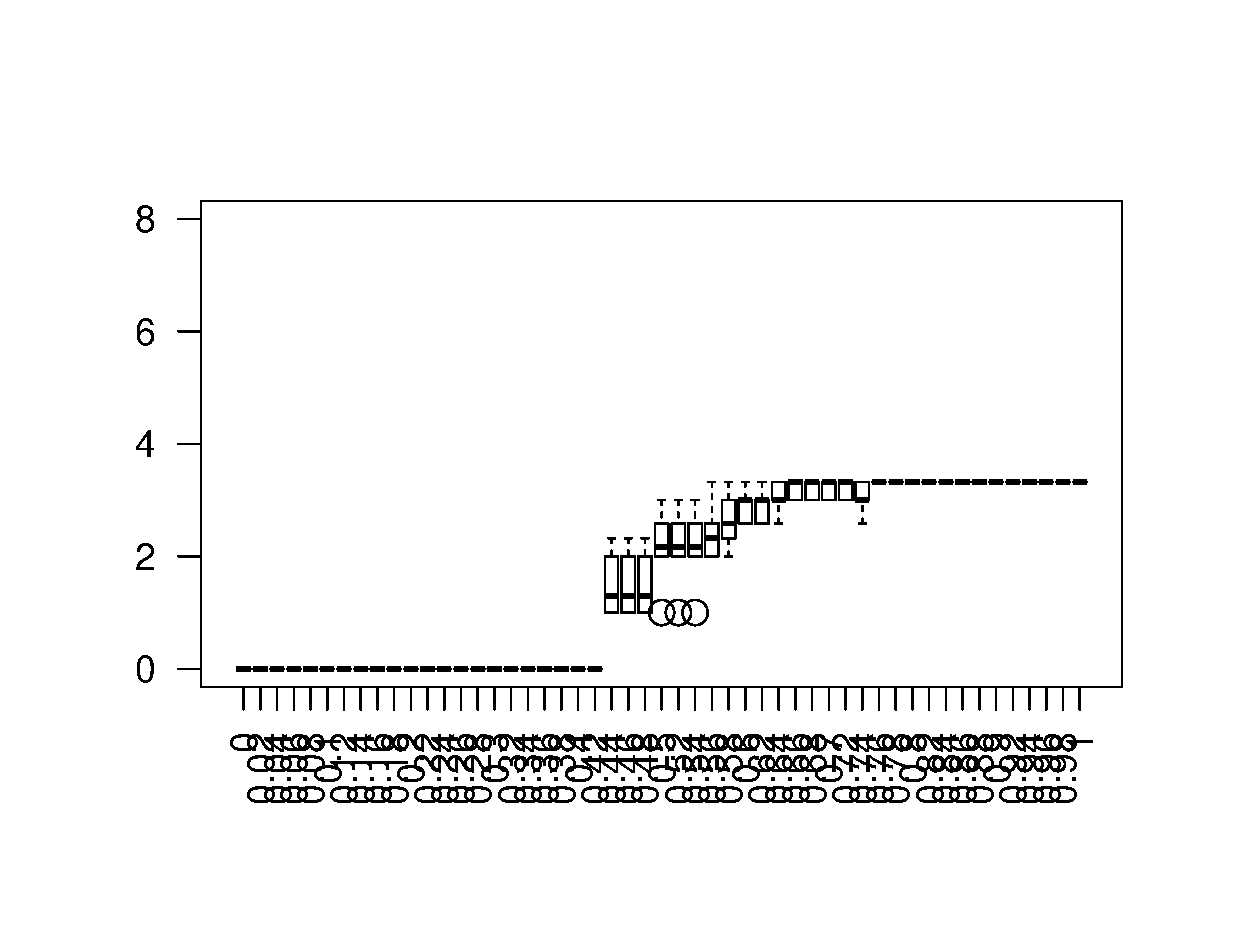
\includegraphics[width=7cm]{n08_chain_large_empsust.eps}}

\centerline{\includegraphics[width=7cm]{n08_chain_large_corr_dss_emp_ai030.eps}}

\centerline{\includegraphics[width=7cm]{n08_chain_large_corr_dss_emp_ai070.eps}}

\centerline{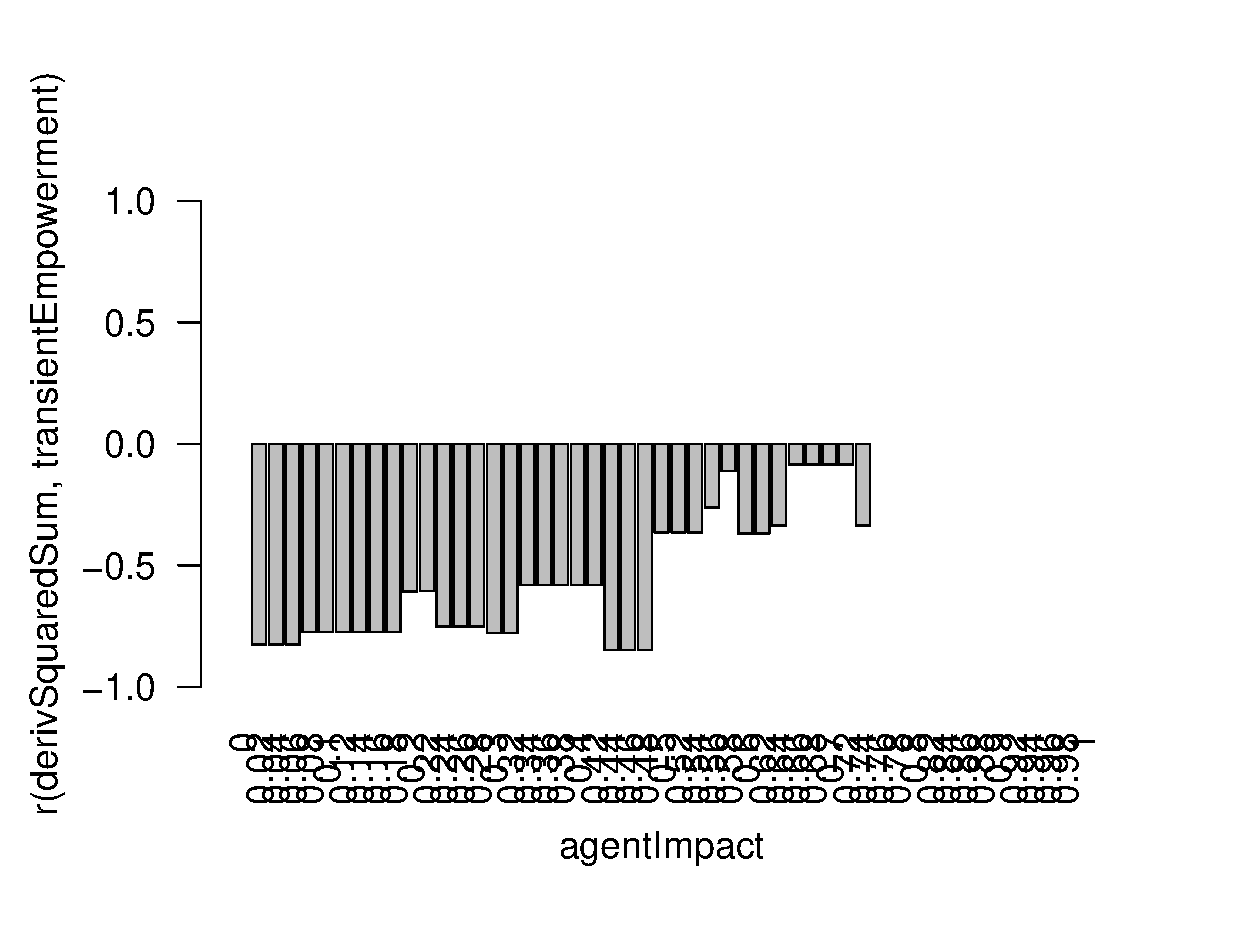
\includegraphics[width=7cm]{n08_chain_large_corr_dss_emp.eps}}

\centerline{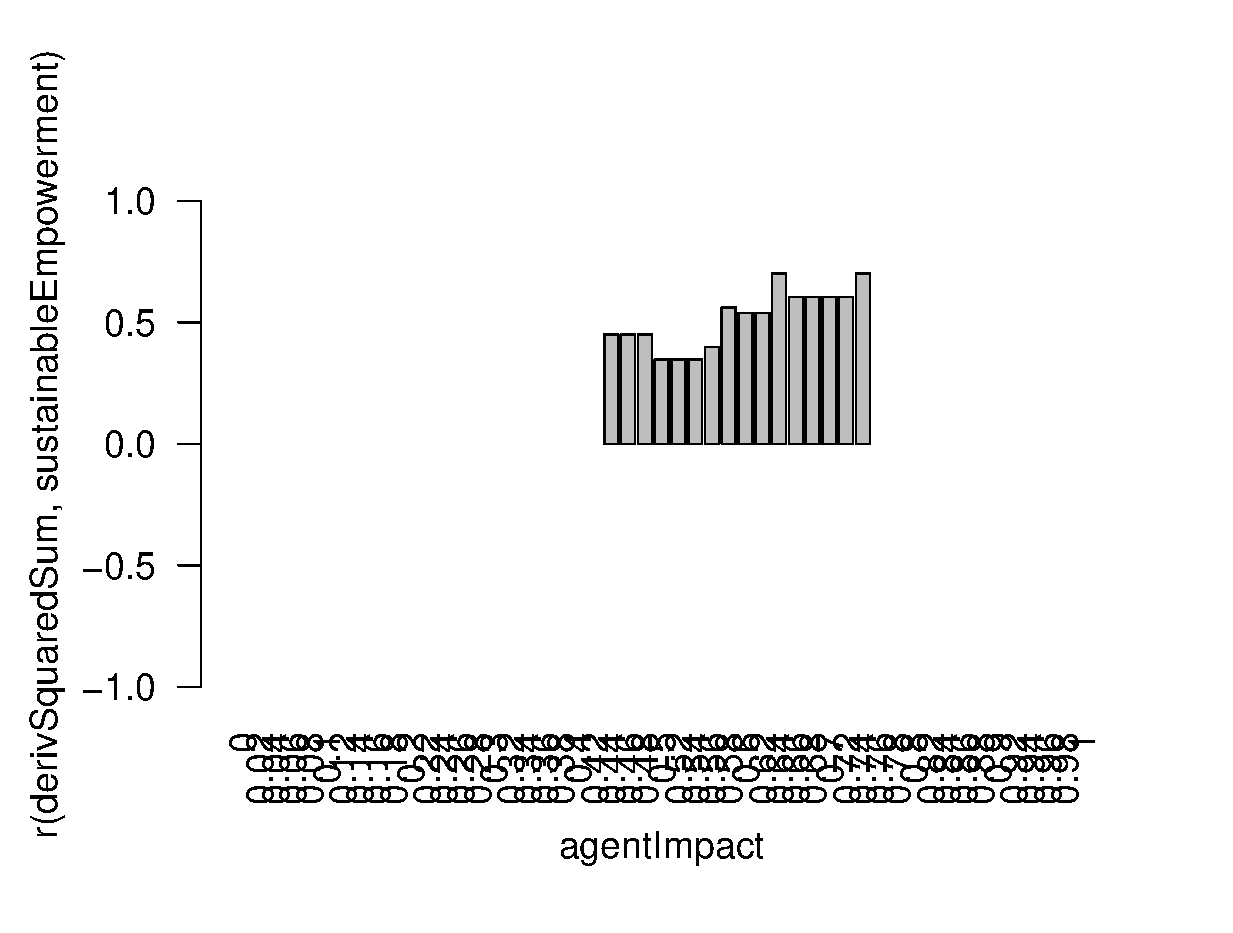
\includegraphics[width=7cm]{n08_chain_large_corr_dss_empsust.eps}}


\cleardoublepage


\subsection{Results (Old)}

We generated the variable parameters $c_i$ and the lower triangle of
$(d_{ji})$ by drawing from uniform distributions. The values of $c_i$
were drawn from $[-0.1, 1]$, and we created an environment with weaker
coupling constants $d_{ji} \in [-0.2, 0.2]$ and one with stronger
coupling constants $d_{ji} \in [-0.8, 2=0.8]$.

Fig.~\ref{fig_empowermentprofiles} shows profiles of empowerment as a
function of $E$, the agent's potential impact on the environment's
tipping elements. At $E = 0$, empowerment is $0$ as the agent is
unable to make any change to the stable state of the environment.
Fig~\ref{fig_empowermentprofiles} shows results for the ``normal''
stable state in which most elements are at $x_{i-}$. Given to the
symmetric method of generating our system's parameters, this
``normal'' is representative for the states of the system in general.

At $E = 0$ the agent has no empowerment, as explained above, and this
extends into small nonzero values of $E$. This is because for an
element in the ``normal'' stable state $x_{i-}$, it is necessary that
$E > \ccrit + C_i$ for the agent to put the element into the
``tipped'' state $x_{i+}$. This explains the emergence of nonzero
empowerment around $E = \ccrit$. Such shifts are somewhat easier with
weaker coupling, which is reflected by the onset of empowerment at
slightly lower $E$.

It is also noticeable from Fig.~\ref{fig_empowermentprofiles} that
weaker coupling enables the agent to attain higher empowerment. One
reason for this is that the number of stable states is maximal in
systems with no coupling at all. In this special case, each element
can be set to each of its two states, independently of all other
elements. At the other end of the scale, a strong interaction from an
upstream element $j$, say with $d_{ji} x_j > \ccrit$, increases the
chance that element $i$ has only one stable state altogether. As a
result, the number of stable system states decreases as the range of
randomly generated $d_{ji}$ increases, explaining also the lower
plateau in empowerment seen with strong coupling.


\subsection{Additional Introductory Notes}

Cubic differential equations are a simple (arguably the simplest)
systems for studying tipping processes. There always is at least one
stable fixed point, i.e.\ one root of the differential equation where
the first derivative is negative, and if the effective intercept is
within a suitable range, two stable fixed points exist, thus enabling
the system to be in two alternative states.

Sustainability has been characterised based on ecosystems properties,
such as existence of fixed points or robustness to perturbations.
While it is clear (or at least entirely plausible) that some form of
stability or robustness is a necessary condition for sustainability,
this condition is not likely sufficient. System states that are very
stable but would not be considered sustainable are easy to construct.
As an example, increasing the average temperature on earth by more
than 5 degrees might well be considered unsustainable even if it could
be shown that the state of the earth's climate system would be very
stable after that amount of global warming. Typical sustainability
concerns put forward in such a scenario include loss of arable land
caused by e.g.\ rising sea levels and desertification. This reveals
that sustainability includes an aspect of providing ``ecosystem
services'' or generating ``natural capital''.

In the past we have introduced the approach of expressly including the
entity, or the agent, which is to be sustained, in a model
\cite{Kim2009_sustainability}. Here, we demonstrate application of
this approach to systems of coupled tipping elements, which have been
established as a simple formalisation of systems for investigating
aspects of stability and sustainability.


\subsection{Additional Discussion Items}

The stability of systems of coupled differential equations has been an
area of interest since decades
\cite{May1972_stablelargecomplexsystem,Landi2018_ecologicalnetworks}.

\cite{May1972_stablelargecomplexsystem} considers a very general
class of dynamic systems, characterised locally by a Jacobian. In this
context, stability is defined by fixed points, whereas other
attractors (cyclic or strange) are considered to represent
instability.

We deliberately restrict coupling to a directed acyclic graph. As a
result, all attractors are fixed points, so in the sense of
\cite{May1972_stablelargecomplexsystem} these systems are always
``stable''.

If elements governed by cubic differential equations are allowed to
mutually impact each other (i.e.\ element $i$ impacts on element $j$
and vice versa), it is rather easy to construct systems in which the
elements do not have any fixed points, but are jointly participating
in a cyclic attractor. As a result, these elements can no longer be
characterised as being in one of two discretisable states
(characterised by fixed points labelled ``sustainable'' and
``tipped'', respectively. From this perspective, coupling of cubic
differential equations with a DAG, as used in this paper, can be
considered to be the most general way of coupling that preserves the
``tipping element'' characteristic of the individual elements.

% summarise system

% perspective of introducing more realistic models of agent impacts
% and constraints, e.g. some natural impact of the agent's /
% humankind's life style etc. and additional costs to mitigate these.

% emphasise generality, coupled tipping elements were chosen as an
% illustrative example, approach of agent interacting with environment
% can be applied very generally

% reiterate accommodation of noise / incomplete information

\end{document}

%%% Local Variables:
%%% mode: latex
%%% TeX-master: t
%%% End:
